\documentclass[11pt,a4paper]{article}

% ---- packages ----
\usepackage[margin=1in]{geometry}
\usepackage{graphicx}
\usepackage{booktabs}
\usepackage{amsmath}
\usepackage{hyperref}
\usepackage{xcolor}
\usepackage{float}
\usepackage{caption}
\usepackage{subcaption}
\usepackage{multirow}
\usepackage{longtable}
\usepackage{array}
\usepackage[numbers,sort&compress]{natbib}
\usepackage{titlesec}

\hypersetup{
    colorlinks=true,
    linkcolor=blue!60!black,
    citecolor=blue!60!black,
    urlcolor=blue!60!black
}

% compact sections
\titlespacing*{\section}{0pt}{1.5ex plus 0.5ex}{0.8ex plus 0.2ex}
\titlespacing*{\subsection}{0pt}{1.2ex plus 0.3ex}{0.6ex plus 0.2ex}

% figure path
\graphicspath{{../results/figures/}}

% shorthand
\newcommand{\pKD}{pK\textsubscript{D}}
\newcommand{\KD}{K\textsubscript{D}}
\newcommand{\ap}{\text{AP}}

\title{\textbf{WillItBind}: Predicting Experimental Binding Success\\from Computational Protein Design Features\\[0.4em]
\large A Meta-Analysis of 5,253 De Novo Designs Across 24 Targets}

\author{Sergio Martinez \\ University of California, Berkeley}

\date{February 2026}

\begin{document}

\maketitle

% ======================================================================
\begin{abstract}
De novo protein binder design has made remarkable progress computationally, but the gap between computational prediction and experimental validation remains poorly understood.
We analyze 5,253 computationally designed proteins tested against 24 targets, expanding the dataset of Overath et al.\ (2025) from 3,766 binders across 15 targets.
Our analysis asks: which computational metrics best predict experimental binding success?
Using Average Precision (AP) as the primary metric for this imbalanced classification task (17.9\% binders), we find that (i) ESMFold pLDDT is the most universally significant single predictor ($p = 6.9 \times 10^{-11}$, Cohen's $d = 0.42$); (ii) pairwise interaction features---products of structural confidence and physicochemical descriptors---improve prediction by 17.3\% over the best individual feature (AP = 0.326 vs.\ 0.278); (iii) per-target AP varies from 0.10 to 0.95, indicating that target tractability dominates over scoring quality; (iv) greedy forward selection converges at just 2 features (charged residue fraction + TM-score, cross-validated AP = 0.61); and (v) sequence identity to known proteins is the strongest predictor of binding affinity among confirmed binders (Spearman $r = 0.68$ with \pKD).
These findings confirm and extend the core conclusions of Overath et al.\ on a larger, more diverse dataset.
Code and results are available at \url{https://github.com/sermare/willitbind}.
\end{abstract}

% ======================================================================
\section{Introduction}

Computational protein design has advanced rapidly, enabling the de novo creation of protein binders against therapeutically relevant targets \cite{overath2025}.
Tools such as RFdiffusion \cite{watson2023}, ProteinMPNN \cite{dauparas2022}, and structure prediction methods including AlphaFold2, ESMFold, and Boltz2 have made it possible to generate thousands of candidate designs in silico.
However, the experimental success rate of these designs remains low: typical campaigns report binding rates of 5--20\%, and the relationship between computational confidence scores and experimental outcomes is not straightforward.

Overath et al.\ (2025) performed the first large-scale meta-analysis of this question, assembling 3,766 experimentally characterized binders across 15 targets.
Their key findings included: (i) structure prediction confidence (specifically ipSAE from AlphaFold3) is the single most predictive feature; (ii) interaction features combining confidence with physicochemical properties outperform individual features; (iii) prediction quality varies dramatically across targets; and (iv) greedy forward selection converges at 2--5 features.

We extend this work using an expanded dataset of 5,253 protein designs evaluated against 24 targets, incorporating predictions from ESMFold, Boltz2, ProteinMPNN, and structural homology searches (Foldseek against AFDB50, PDB100, and CATH50), paired with experimental binding data (\KD, $k_{\text{on}}$, $k_{\text{off}}$) from surface plasmon resonance (SPR) and bio-layer interferometry (BLI).

Our analysis replicates and extends the Overath et al.\ methodology on this larger dataset, confirming their core conclusions while revealing additional insights about feature consistency across targets and the role of sequence-derived physicochemical properties.

% ======================================================================
\section{Dataset}

\subsection{Overview}

The dataset comprises 5,253 computationally designed proteins with JSON-encoded evaluation records spanning computational predictions and experimental measurements.
After parsing into a long-format analysis dataset (one row per protein-target pair), we obtain 2,630 evaluable pairs across 24 unique targets, of which 470 (17.9\%) are experimentally confirmed binders.

\begin{table}[H]
\centering
\caption{Dataset summary statistics.}
\label{tab:dataset}
\begin{tabular}{lr}
\toprule
Statistic & Value \\
\midrule
Total protein designs & 5,253 \\
Protein-target pairs with binding data & 2,630 \\
Experimentally confirmed binders & 470 (17.9\%) \\
Unique targets & 24 \\
Computational features analyzed & 49 \\
Targets with $>$50 samples & 5 \\
Binding rate range across targets & 0\%--70\% \\
\bottomrule
\end{tabular}
\end{table}

\subsection{Data leakage prevention}

A critical methodological concern in this analysis is the separation of computational features (predictors) from experimental labels (ground truth).
Features derived from experimental binding measurements (e.g., measured \KD, $k_{\text{on}}$, $k_{\text{off}}$) are strictly excluded from the predictor set.
Only features available before experimental testing---structure prediction confidence, sequence properties, and homology search results---are used as predictors.
Binding status (binder vs.\ non-binder) and binding affinity (\pKD) serve as response variables.

\subsection{Feature categories}

We analyze 49 computational features organized into four categories:

\begin{enumerate}
    \item \textbf{Structure prediction confidence} (7 features): ESMFold pLDDT, Boltz2 complex iPLDDT, Boltz2 pLDDT, shape complementarity, Boltz2 ipSAE, Boltz2 LIS, and TED confidence.

    \item \textbf{Sequence design scores} (4 features): ProteinMPNN score, ProteinMPNN sequence recovery, redesigned ProteinMPNN score, and sequence identity to template.

    \item \textbf{Structural homology} (18 features): TM-scores, RMSD, e-values, aligned lengths, and sequence identities from Foldseek searches against AFDB50, PDB100, and CATH50.

    \item \textbf{Sequence-derived physicochemical properties} (10 features): molecular weight, GRAVY index, fraction polar/hydrophobic/aromatic/charged residues, charge density, net charge, and sequence length.

    \item \textbf{Domain match features} (10 features): Domain-level e-values, RMSD, TM-scores, aligned lengths, and sequence identities from AFDB50 domain matching.
\end{enumerate}

\subsection{Target diversity}

The 24 targets span a wide range of biological functions and structural classes (Table~\ref{tab:targets}).
Binding rates vary from 0\% (human-serum-albumin, human-tnfa, human-gm2a, human-orm2) to 70\% (spcas9), reflecting dramatic differences in target tractability.

\begin{table}[H]
\centering
\caption{Per-target summary for targets with at least 20 samples. Shown are the number of samples ($n$), number of binders, binding rate, and the Cohen's $d$ effect size for the top-ranked feature.}
\label{tab:targets}
\begin{tabular}{lrrrr}
\toprule
Target & $n$ & Binders & Rate (\%) & Top $|d|$ \\
\midrule
nipah-glycoprotein-g & 1,033 & 103 & 10.0 & 0.670 \\
egfr & 770 & 129 & 16.8 & --- \\
il7r & 97 & 62 & 63.9 & 0.618 \\
human-serum-albumin & 103 & 0 & 0.0 & --- \\
pd-l1 & 75 & 39 & 52.0 & --- \\
human-insulin-receptor & 35 & 21 & 60.0 & 1.184 \\
human-tnfa & 35 & 0 & 0.0 & --- \\
human-pdgfr-beta & 30 & 18 & 60.0 & 0.646 \\
human-mzb1-perp1 & 30 & 15 & 50.0 & 2.974 \\
human-pmvk & 30 & 10 & 33.3 & --- \\
fcrn & 24 & 6 & 25.0 & 1.342 \\
mdm2 & 22 & 6 & 27.3 & --- \\
spcas9 & 20 & 14 & 70.0 & --- \\
\bottomrule
\end{tabular}
\end{table}

% ======================================================================
\section{Methods}

\subsection{Statistical testing}

For each computational feature, we perform a two-sided Mann-Whitney U test comparing the distributions in binders versus non-binders.
Effect sizes are quantified using Cohen's $d$:
\begin{equation}
d = \frac{\bar{x}_{\text{binder}} - \bar{x}_{\text{nonbinder}}}{s_{\text{pooled}}}
\end{equation}
where $s_{\text{pooled}}$ is the pooled standard deviation.
Features with $p < 0.05$ after Bonferroni correction are considered statistically significant.

\subsection{Average Precision}

Following Overath et al., we use Average Precision (AP) as the primary evaluation metric rather than AUC-ROC, since AP is more informative for imbalanced datasets \cite{saito2015}.
For each feature, we compute AP in both directions (higher-is-better and lower-is-better) and report the maximum:
\begin{equation}
\ap = \sum_{k=1}^{n} P(k) \cdot \Delta r(k)
\end{equation}
where $P(k)$ is precision at rank $k$ and $\Delta r(k)$ is the change in recall from rank $k-1$ to $k$.

\subsection{Interaction features}

Following Overath et al., who found that products of confidence metrics and physicochemical descriptors improve prediction, we compute pairwise products of the top 15 individual features.
For features $f_i$ and $f_j$, the interaction feature is $f_i \times f_j$.
AP is computed for each interaction and compared against the best individual AP.

\subsection{LASSO feature selection}

We apply L1-regularized logistic regression (LASSO) for binary binding prediction:
\begin{equation}
\min_{\beta} \left[ -\frac{1}{n} \sum_{i=1}^{n} \left( y_i \log p_i + (1-y_i) \log(1-p_i) \right) + C^{-1} \|\beta\|_1 \right]
\end{equation}
where $C$ controls the regularization strength.
We search $C \in [10^{-4}, 10^{2}]$ using 30 logarithmically spaced values with 5-fold cross-validation, balanced class weights, and a maximum of 5,000 iterations.

For affinity prediction, we apply LassoCV with 10-fold cross-validation to predict \pKD\ among confirmed binders.

\subsection{Greedy forward feature selection}

We implement greedy forward selection with Leave-One-Group-Out cross-validation (LOGO-CV), where each target serves as a held-out group.
At each step, the feature that maximally improves cross-validated AP is added.
Selection terminates when the AP improvement falls below $\Delta\ap = 0.002$.
This mirrors the Overath et al.\ approach and ensures that selected features generalize across targets rather than overfitting to the most populated target.

\subsection{Model training and evaluation}

The final model uses L1-regularized logistic regression with balanced class weights trained on LASSO-selected features.
Threshold optimization maximizes the F1 score.
Enrichment curves report precision at top-$k$ to assess practical utility for experimental prioritization.

% ======================================================================
\section{Results}

\subsection{Binder vs.\ non-binder statistical comparison}

Of 49 features tested, 26 achieve statistical significance at $p < 0.05$ in the Mann-Whitney U test (Figure~\ref{fig:effectsizes}).
The three largest effect sizes are all Boltz2-derived metrics for the nipah-glycoprotein-g target: complex iPLDDT ($d = 0.61$), shape complementarity ($d = 0.55$), and pLDDT ($d = 0.50$).

\begin{figure}[H]
\centering
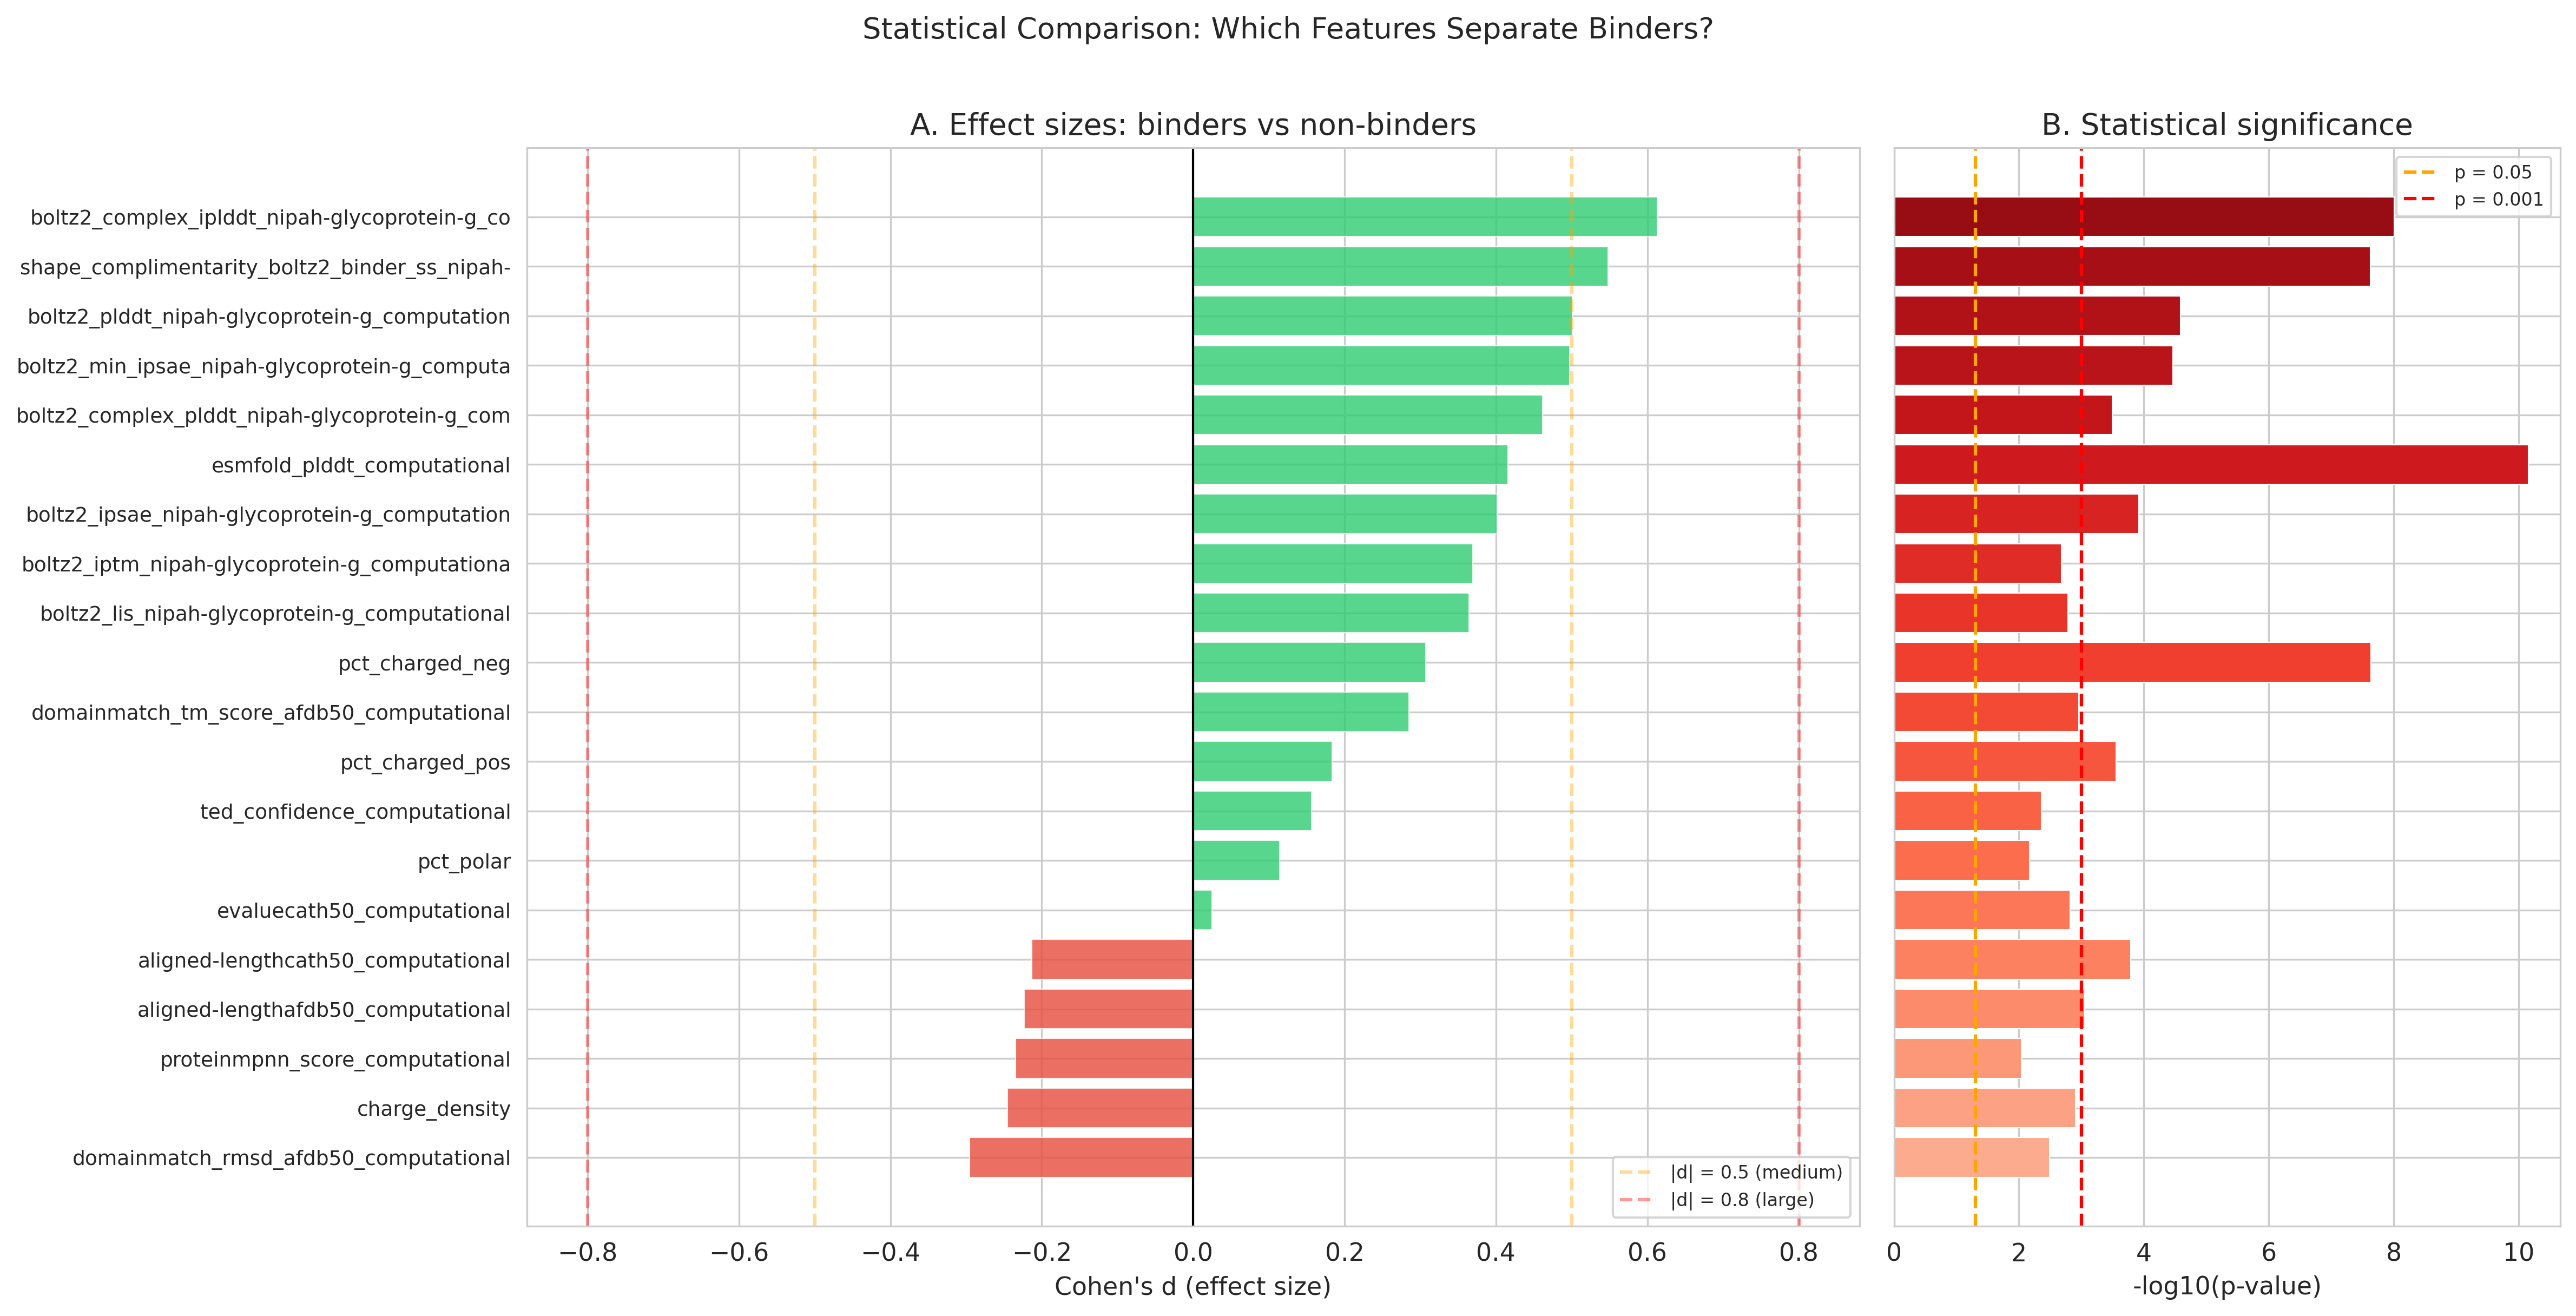
\includegraphics[width=\textwidth]{fig2_effect_sizes.png}
\caption{Cohen's $d$ effect sizes with $-\log_{10}(p)$ annotations for features with $|d| > 0.1$. Positive values indicate higher values in binders. The three largest effects are Boltz2-derived confidence metrics.}
\label{fig:effectsizes}
\end{figure}

ESMFold pLDDT is the most universally significant predictor, achieving $p = 6.9 \times 10^{-11}$ and $d = +0.42$ across all 2,622 evaluable protein-target pairs.
This confirms the finding from Overath et al.\ that structure prediction confidence is the most reliable single indicator of binding success, though on our expanded dataset ESMFold pLDDT takes the lead over AlphaFold3 ipSAE (which was not available for all targets in our dataset).

The volcano plot (Figure~\ref{fig:volcano}) integrates statistical and practical significance, revealing that the most actionable features---those in the upper corners---combine large effect sizes with high confidence.

\begin{figure}[H]
\centering
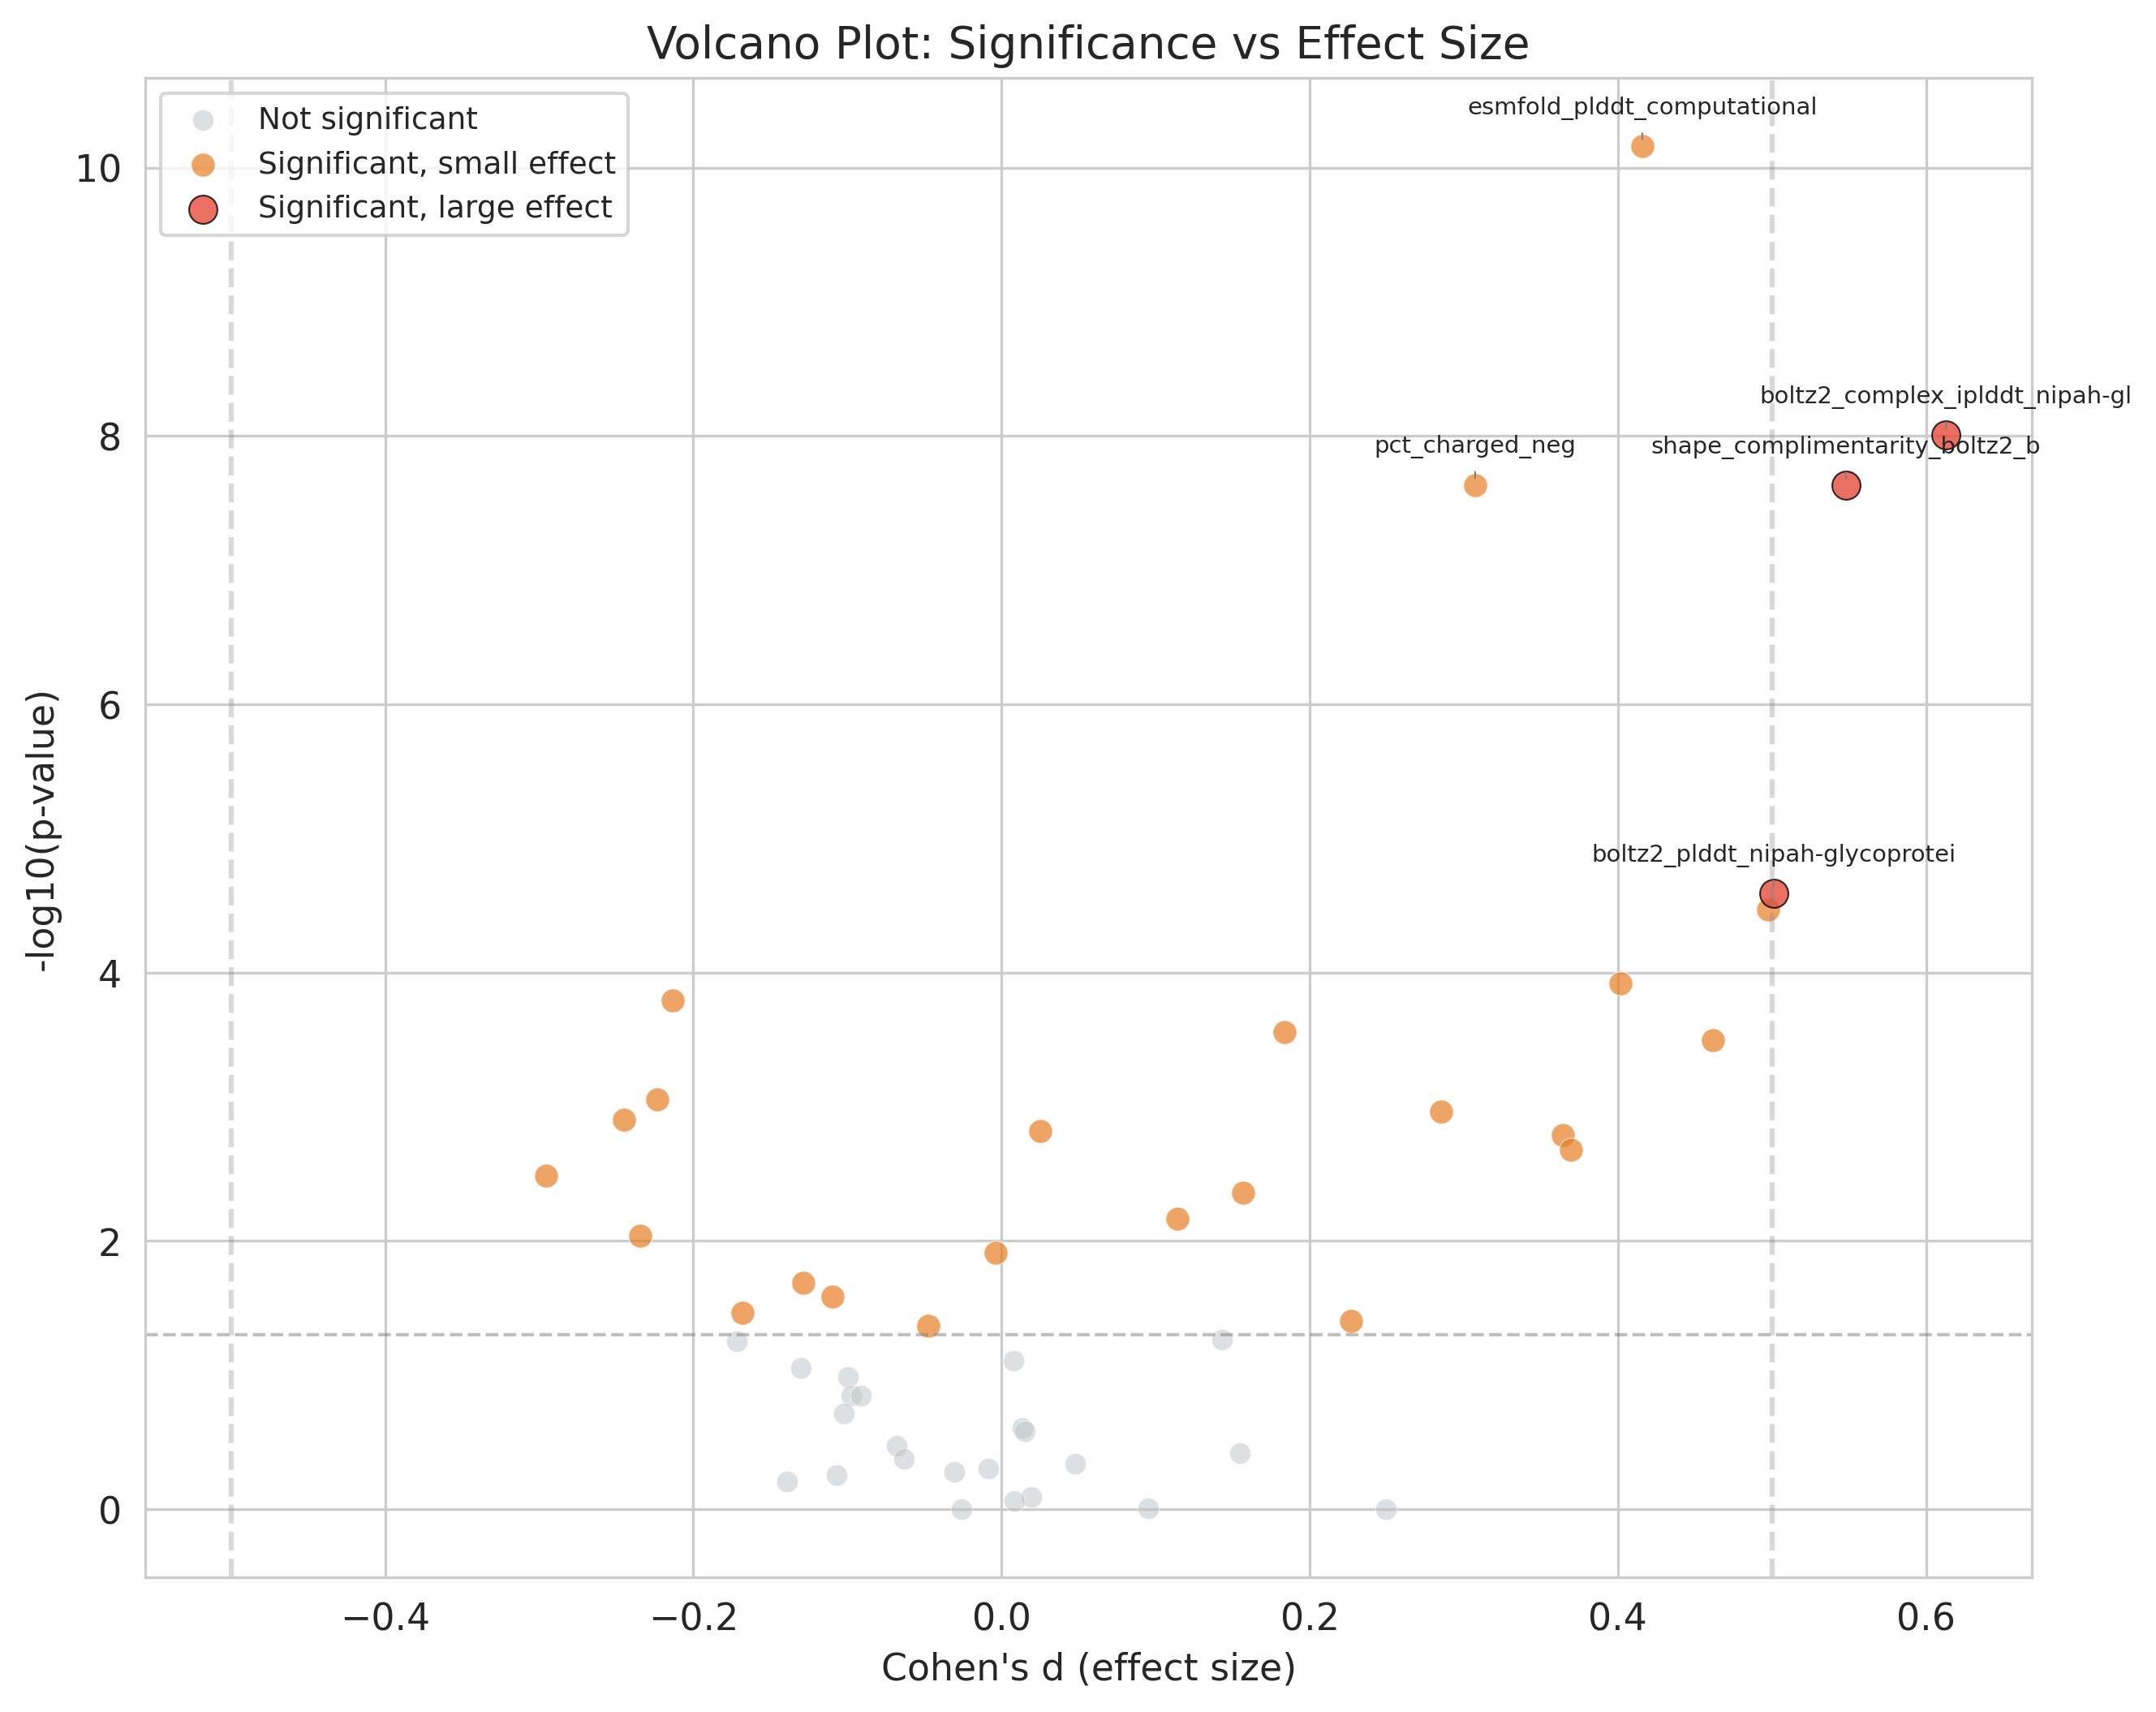
\includegraphics[width=0.85\textwidth]{fig3_volcano.png}
\caption{Volcano plot showing $-\log_{10}(p)$ versus Cohen's $d$ for all 49 features. Features in the upper corners are both statistically and practically significant. Dashed lines indicate $p = 0.05$ (horizontal) and $|d| = 0.2$ (vertical).}
\label{fig:volcano}
\end{figure}

Distribution differences are visible in the violin plots for the top six discriminative features (Figure~\ref{fig:violins}), though substantial overlap is present in all cases---no single feature cleanly separates binders from non-binders.

\begin{figure}[H]
\centering
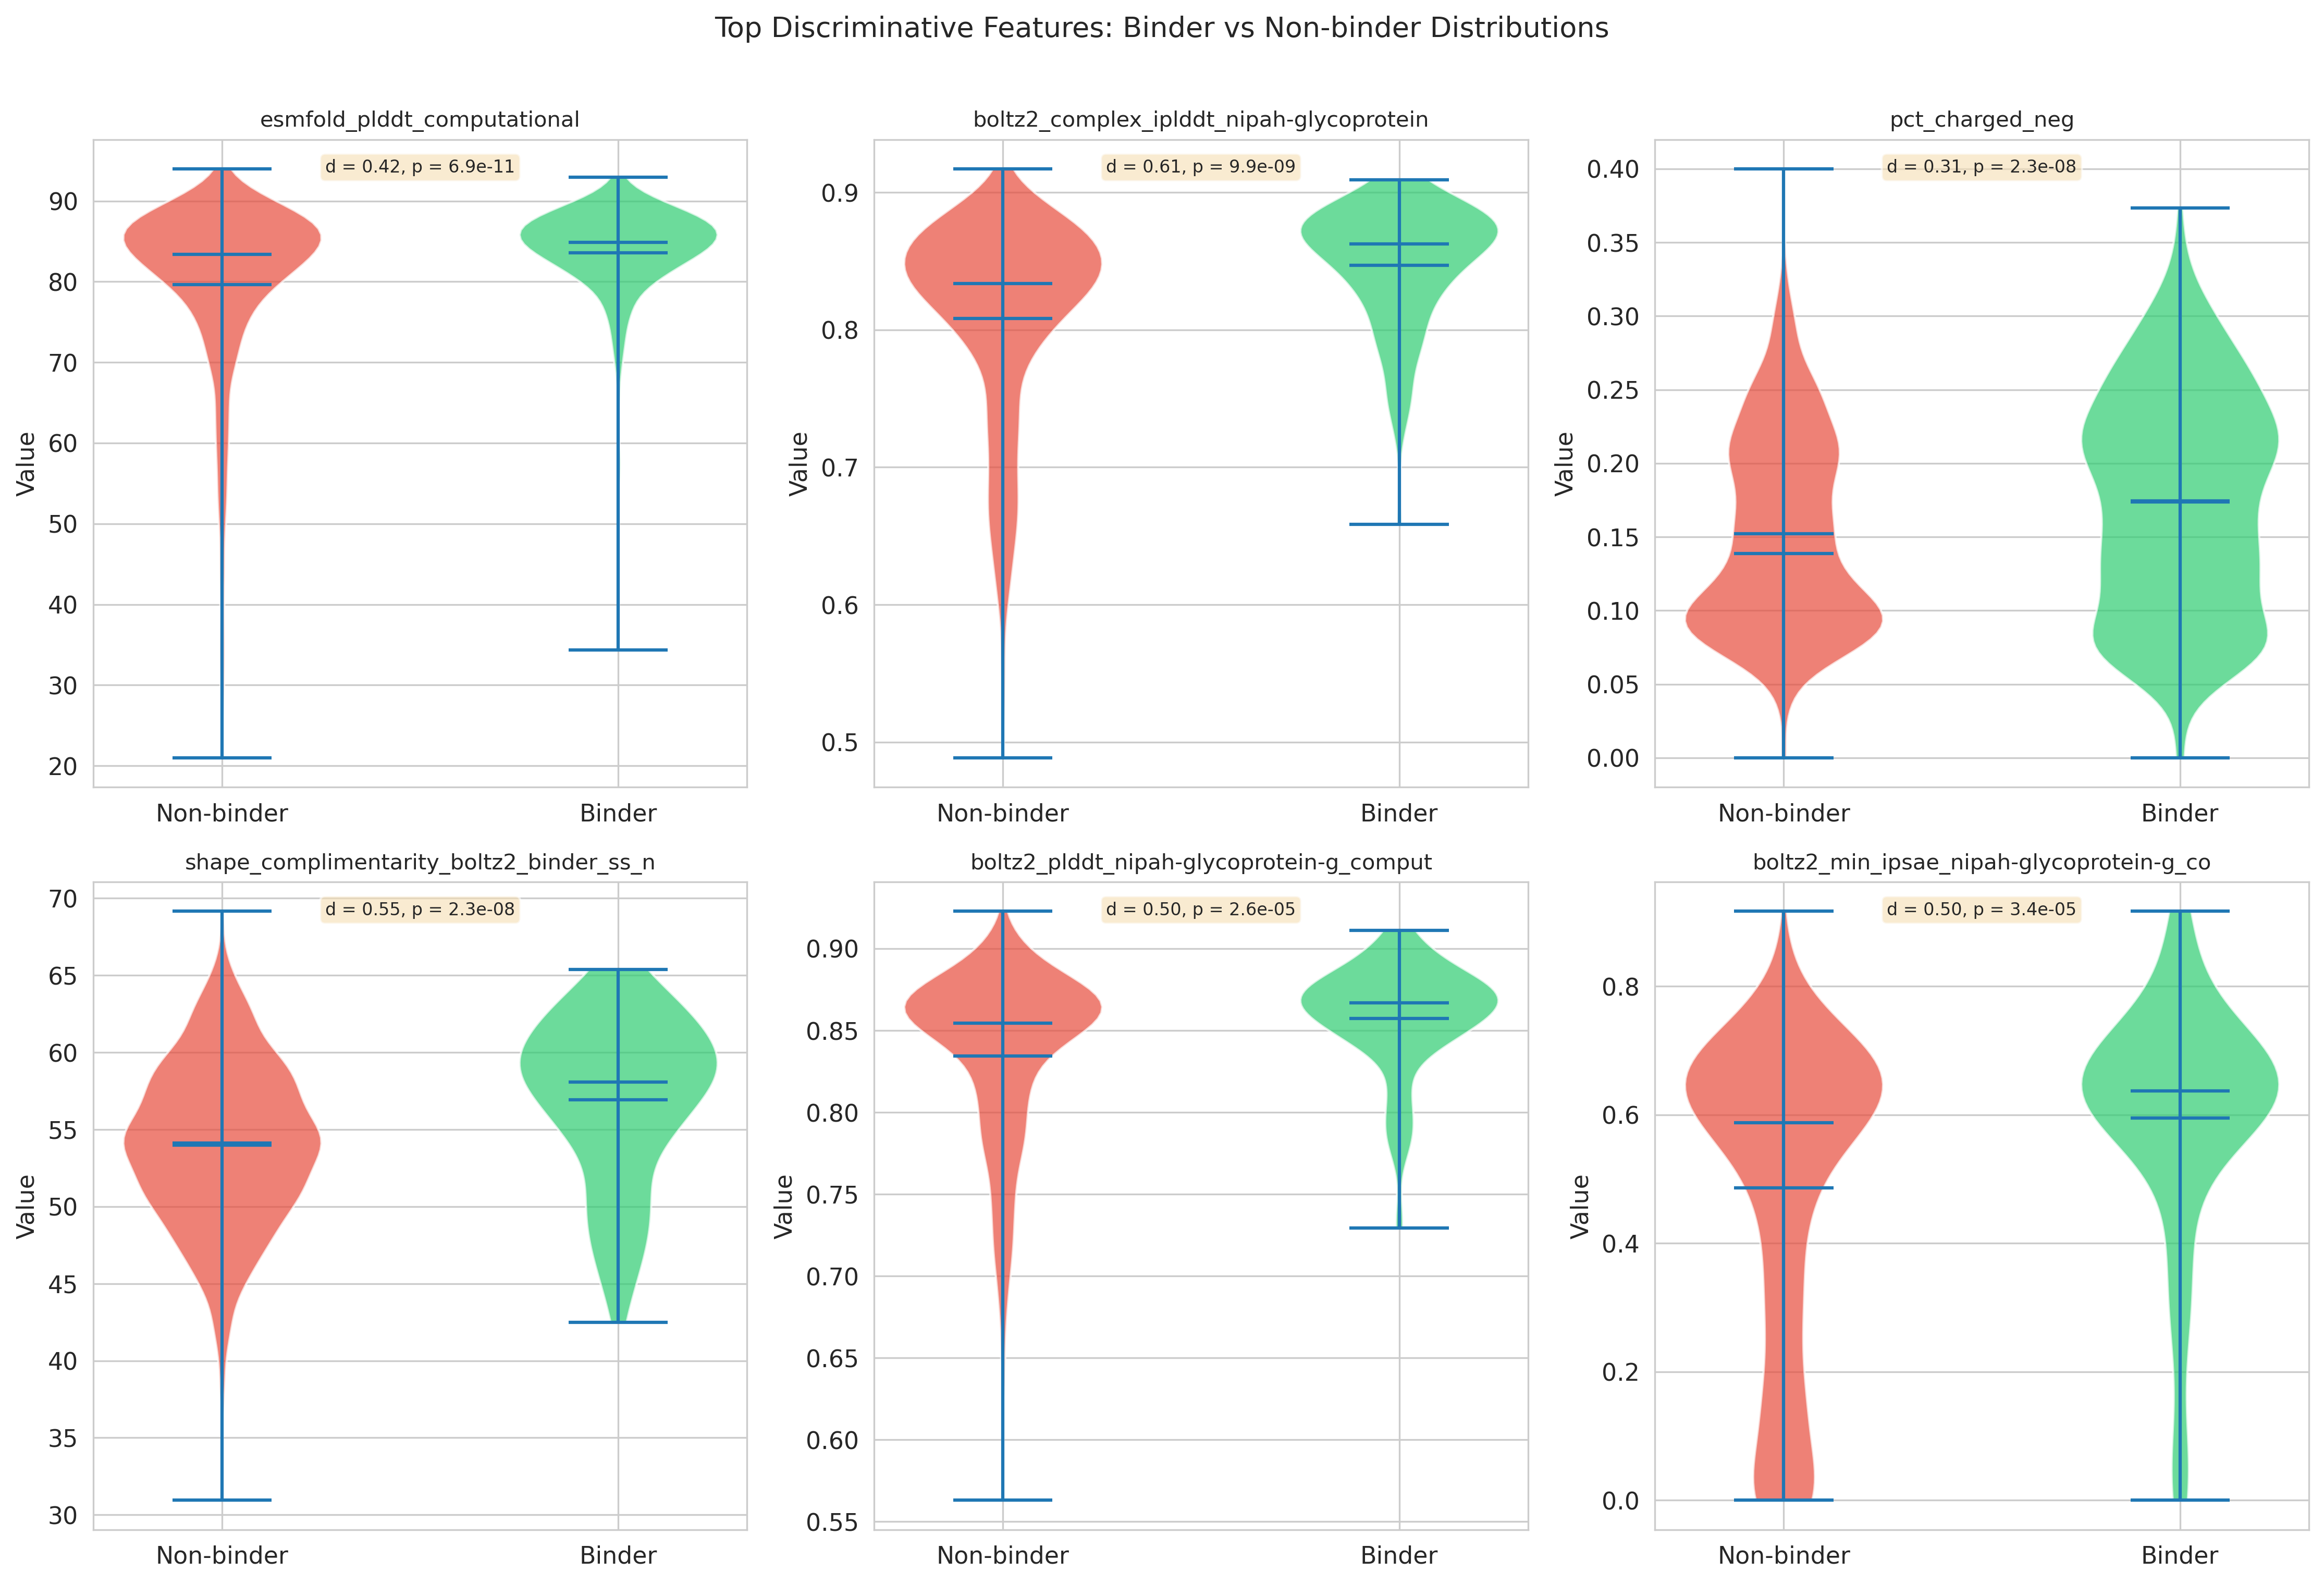
\includegraphics[width=\textwidth]{fig5_top_violins.png}
\caption{Violin plots comparing binder (green) and non-binder (red) distributions for the six most discriminative features. Overlap is substantial for all features.}
\label{fig:violins}
\end{figure}

\subsection{Single feature Average Precision ranking}

Table~\ref{tab:singleap} shows the top 15 features ranked by AP.
The best single feature is aligned-length from CATH50 (AP = 0.278), followed by RMSD from AFDB50 (AP = 0.266) and aligned-length from PDB100 (AP = 0.259).
Notably, many structural homology features (TM-scores, e-values, sequence identities) cluster in the 0.25--0.28 AP range, suggesting substantial redundancy.

\begin{table}[H]
\centering
\caption{Top 15 features ranked by Average Precision. ``Direction'' indicates whether higher or lower values predict binding.}
\label{tab:singleap}
\begin{tabular}{lccr}
\toprule
Feature & AP & Direction & $n$ \\
\midrule
aligned-length (CATH50) & 0.278 & lower & 1,649 \\
RMSD (AFDB50) & 0.266 & lower & 1,645 \\
aligned-length (PDB100) & 0.259 & lower & 1,637 \\
seq.\ identity (PDB100) & 0.259 & higher & 1,637 \\
TM-score (CATH50) & 0.256 & lower & 1,649 \\
TM-score (AFDB50) & 0.256 & higher & 1,645 \\
e-value (CATH50) & 0.256 & higher & 1,649 \\
aligned-length (AFDB50) & 0.254 & lower & 1,645 \\
e-value (AFDB50) & 0.254 & higher & 1,645 \\
RMSD (PDB100) & 0.252 & lower & 1,637 \\
seq.\ identity (AFDB50) & 0.250 & higher & 1,645 \\
TM-score (PDB100) & 0.249 & higher & 1,637 \\
seq.\ identity (CATH50) & 0.249 & higher & 1,649 \\
\% charged neg.\ & 0.235 & higher & 2,630 \\
ESMFold pLDDT & 0.222 & higher & 2,622 \\
\bottomrule
\end{tabular}
\end{table}

\begin{figure}[H]
\centering
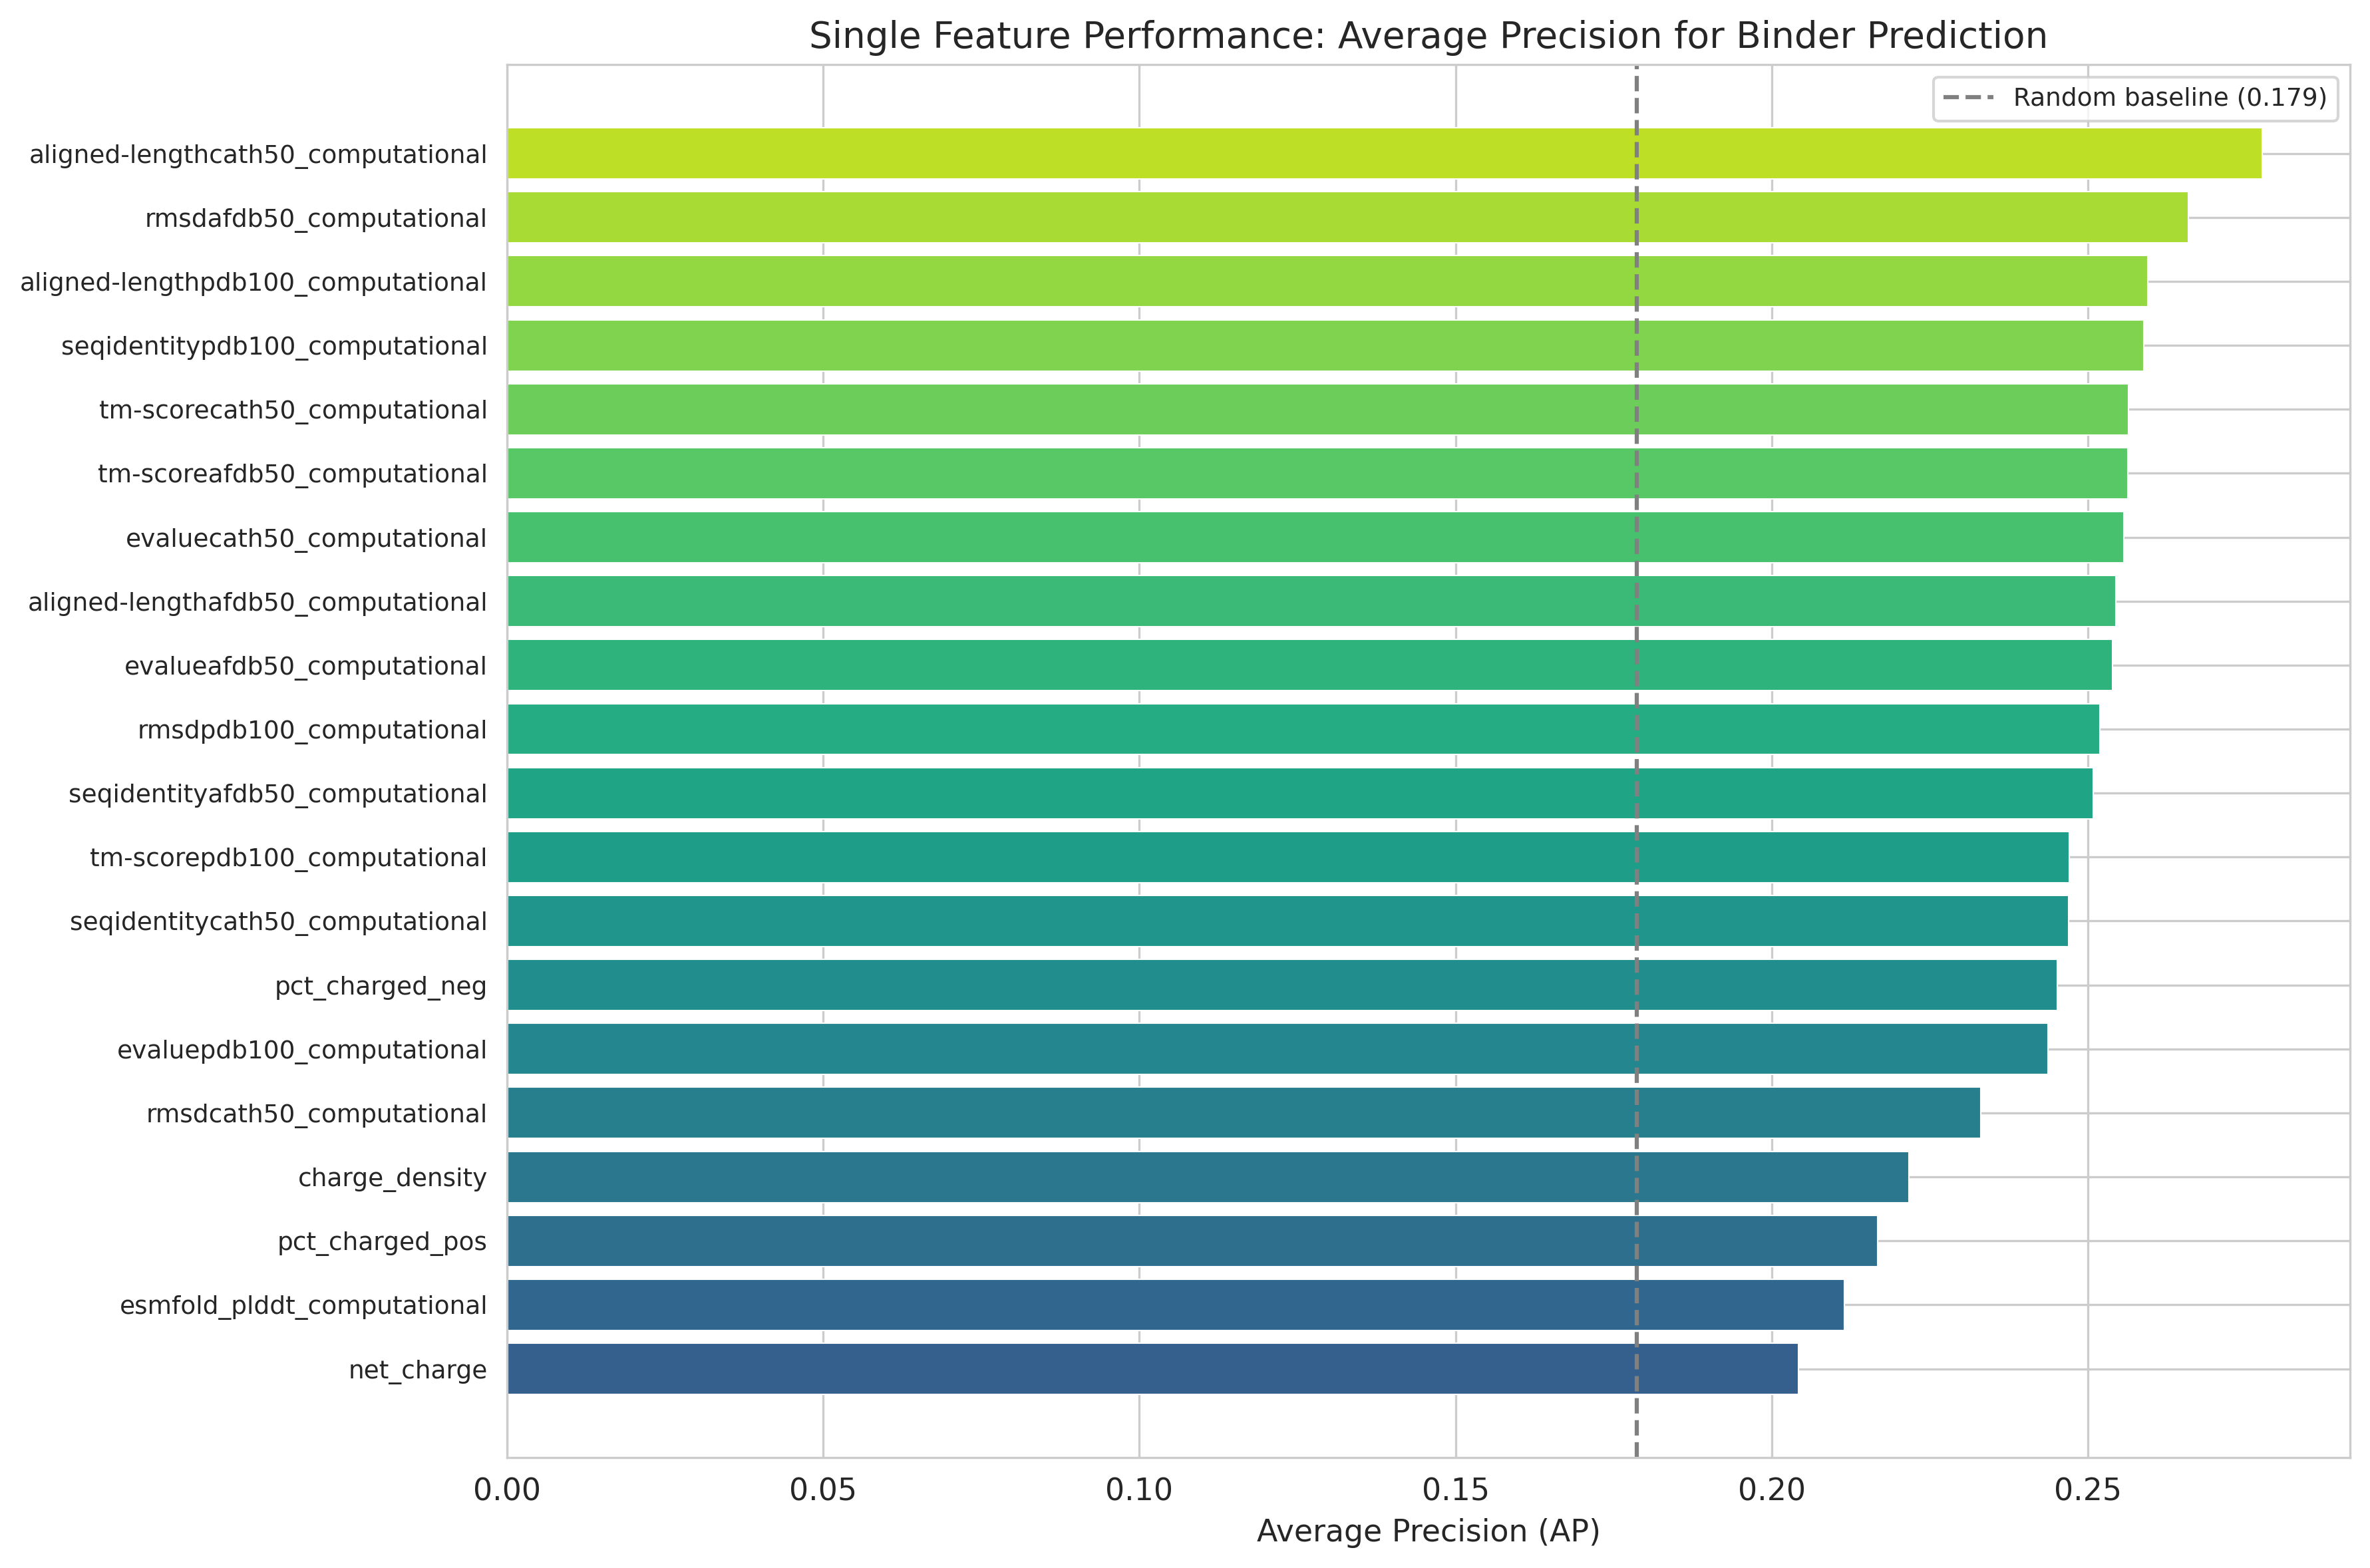
\includegraphics[width=\textwidth]{fig16_single_feature_ap.png}
\caption{Average Precision ranking for all features. Structural homology features dominate the top ranks, with physicochemical and confidence features following.}
\label{fig:singleap}
\end{figure}

\subsection{Interaction features}

Pairwise products of the top 15 features reveal substantial improvements over individual features (Table~\ref{tab:interaction}, Figure~\ref{fig:interaction}).
The best interaction---TM-score (AFDB50) $\times$ negative charge fraction---achieves AP = 0.326, a 17.3\% improvement over the best individual feature (AP = 0.278).

\begin{table}[H]
\centering
\caption{Top 10 interaction features ranked by AP. ``Gain'' is the percentage improvement over the best individual AP (0.278).}
\label{tab:interaction}
\begin{tabular}{lcc}
\toprule
Interaction & AP & Gain (\%) \\
\midrule
TM-score (AFDB50) $\times$ \% charged neg. & 0.326 & +17.3 \\
TM-score (PDB100) $\times$ \% charged neg. & 0.306 & +10.1 \\
TM-score (CATH50) $\times$ \% charged neg. & 0.293 & +5.4 \\
RMSD (PDB100) $\times$ \% charged neg. & 0.288 & +3.6 \\
seq.\ identity (AFDB50) $\times$ \% charged neg. & 0.288 & +3.6 \\
aligned-length (PDB100) $\times$ \% charged neg. & 0.282 & +1.4 \\
RMSD (AFDB50) $\times$ seq.\ identity (AFDB50) & 0.281 & +1.1 \\
RMSD (AFDB50) $\times$ TM-score (CATH50) & 0.281 & +1.1 \\
\bottomrule
\end{tabular}
\end{table}

\begin{figure}[H]
\centering
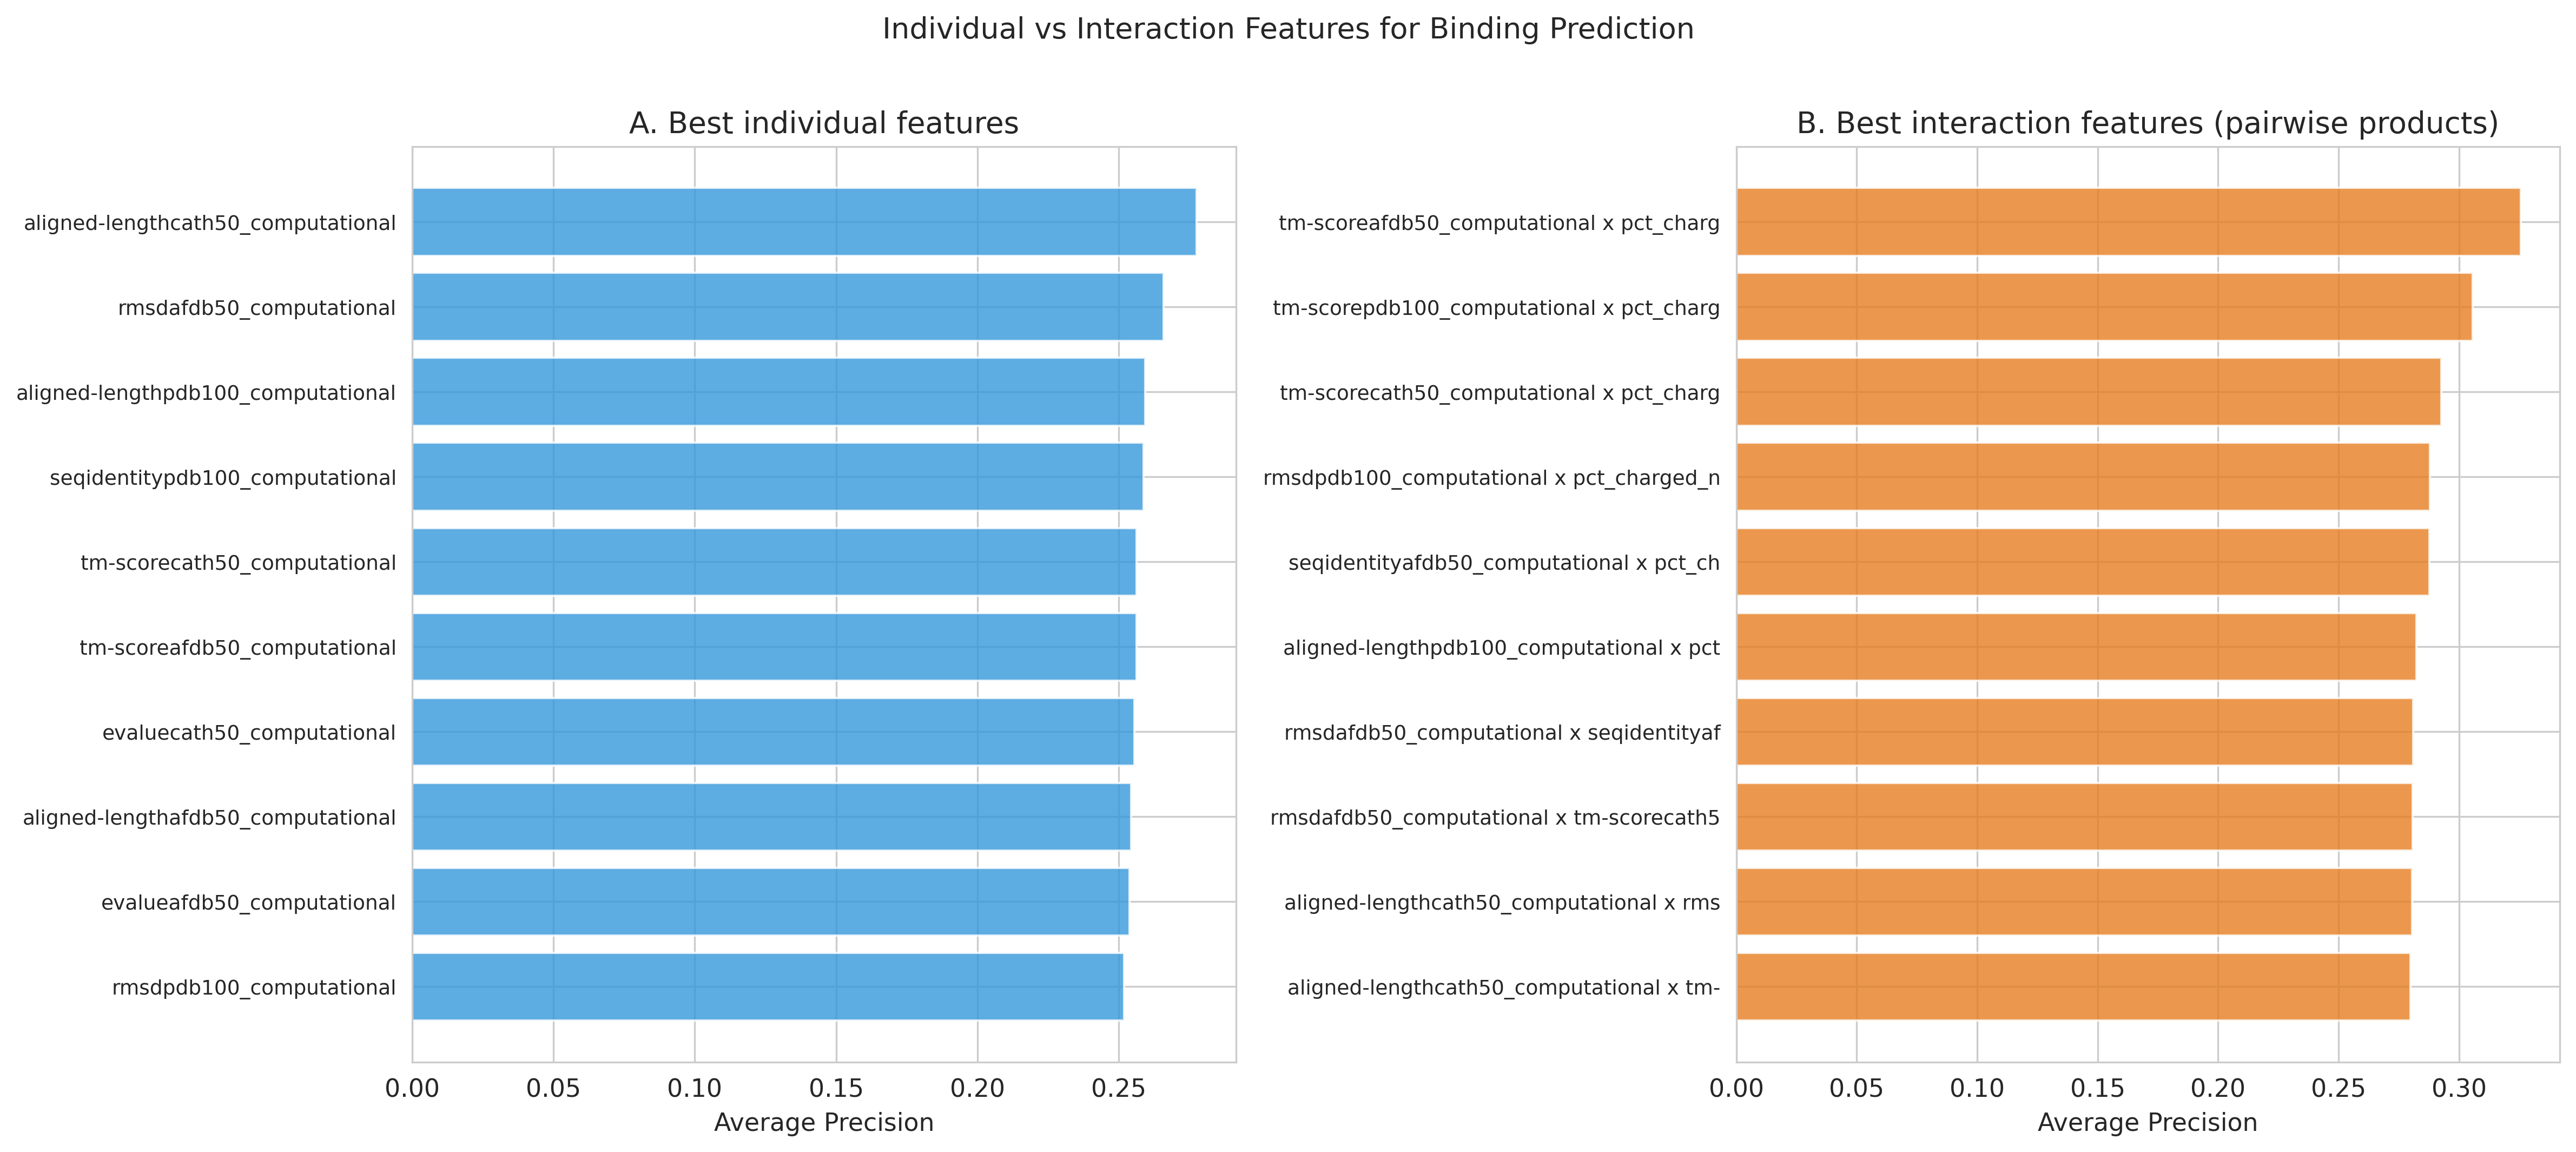
\includegraphics[width=\textwidth]{fig17_interaction_features.png}
\caption{Comparison of individual features (blue) versus interaction features (orange). The best interaction achieves AP = 0.326, substantially outperforming the best individual feature.}
\label{fig:interaction}
\end{figure}

This confirms the key finding from Overath et al.: combining structural confidence metrics with physicochemical descriptors captures complementary information that neither class captures alone.
Notably, the negative charge fraction appears in 6 of the top 8 interactions, suggesting it provides orthogonal information to structure-based metrics.

\subsection{Per-target analysis}

Per-target AP for the best feature ranges from 0.095 (hnmt) to 0.948 (human-mzb1-perp1), consistent with the 0.1--1.0 range reported by Overath et al.\ (Figure~\ref{fig:pertarget}).

\begin{figure}[H]
\centering
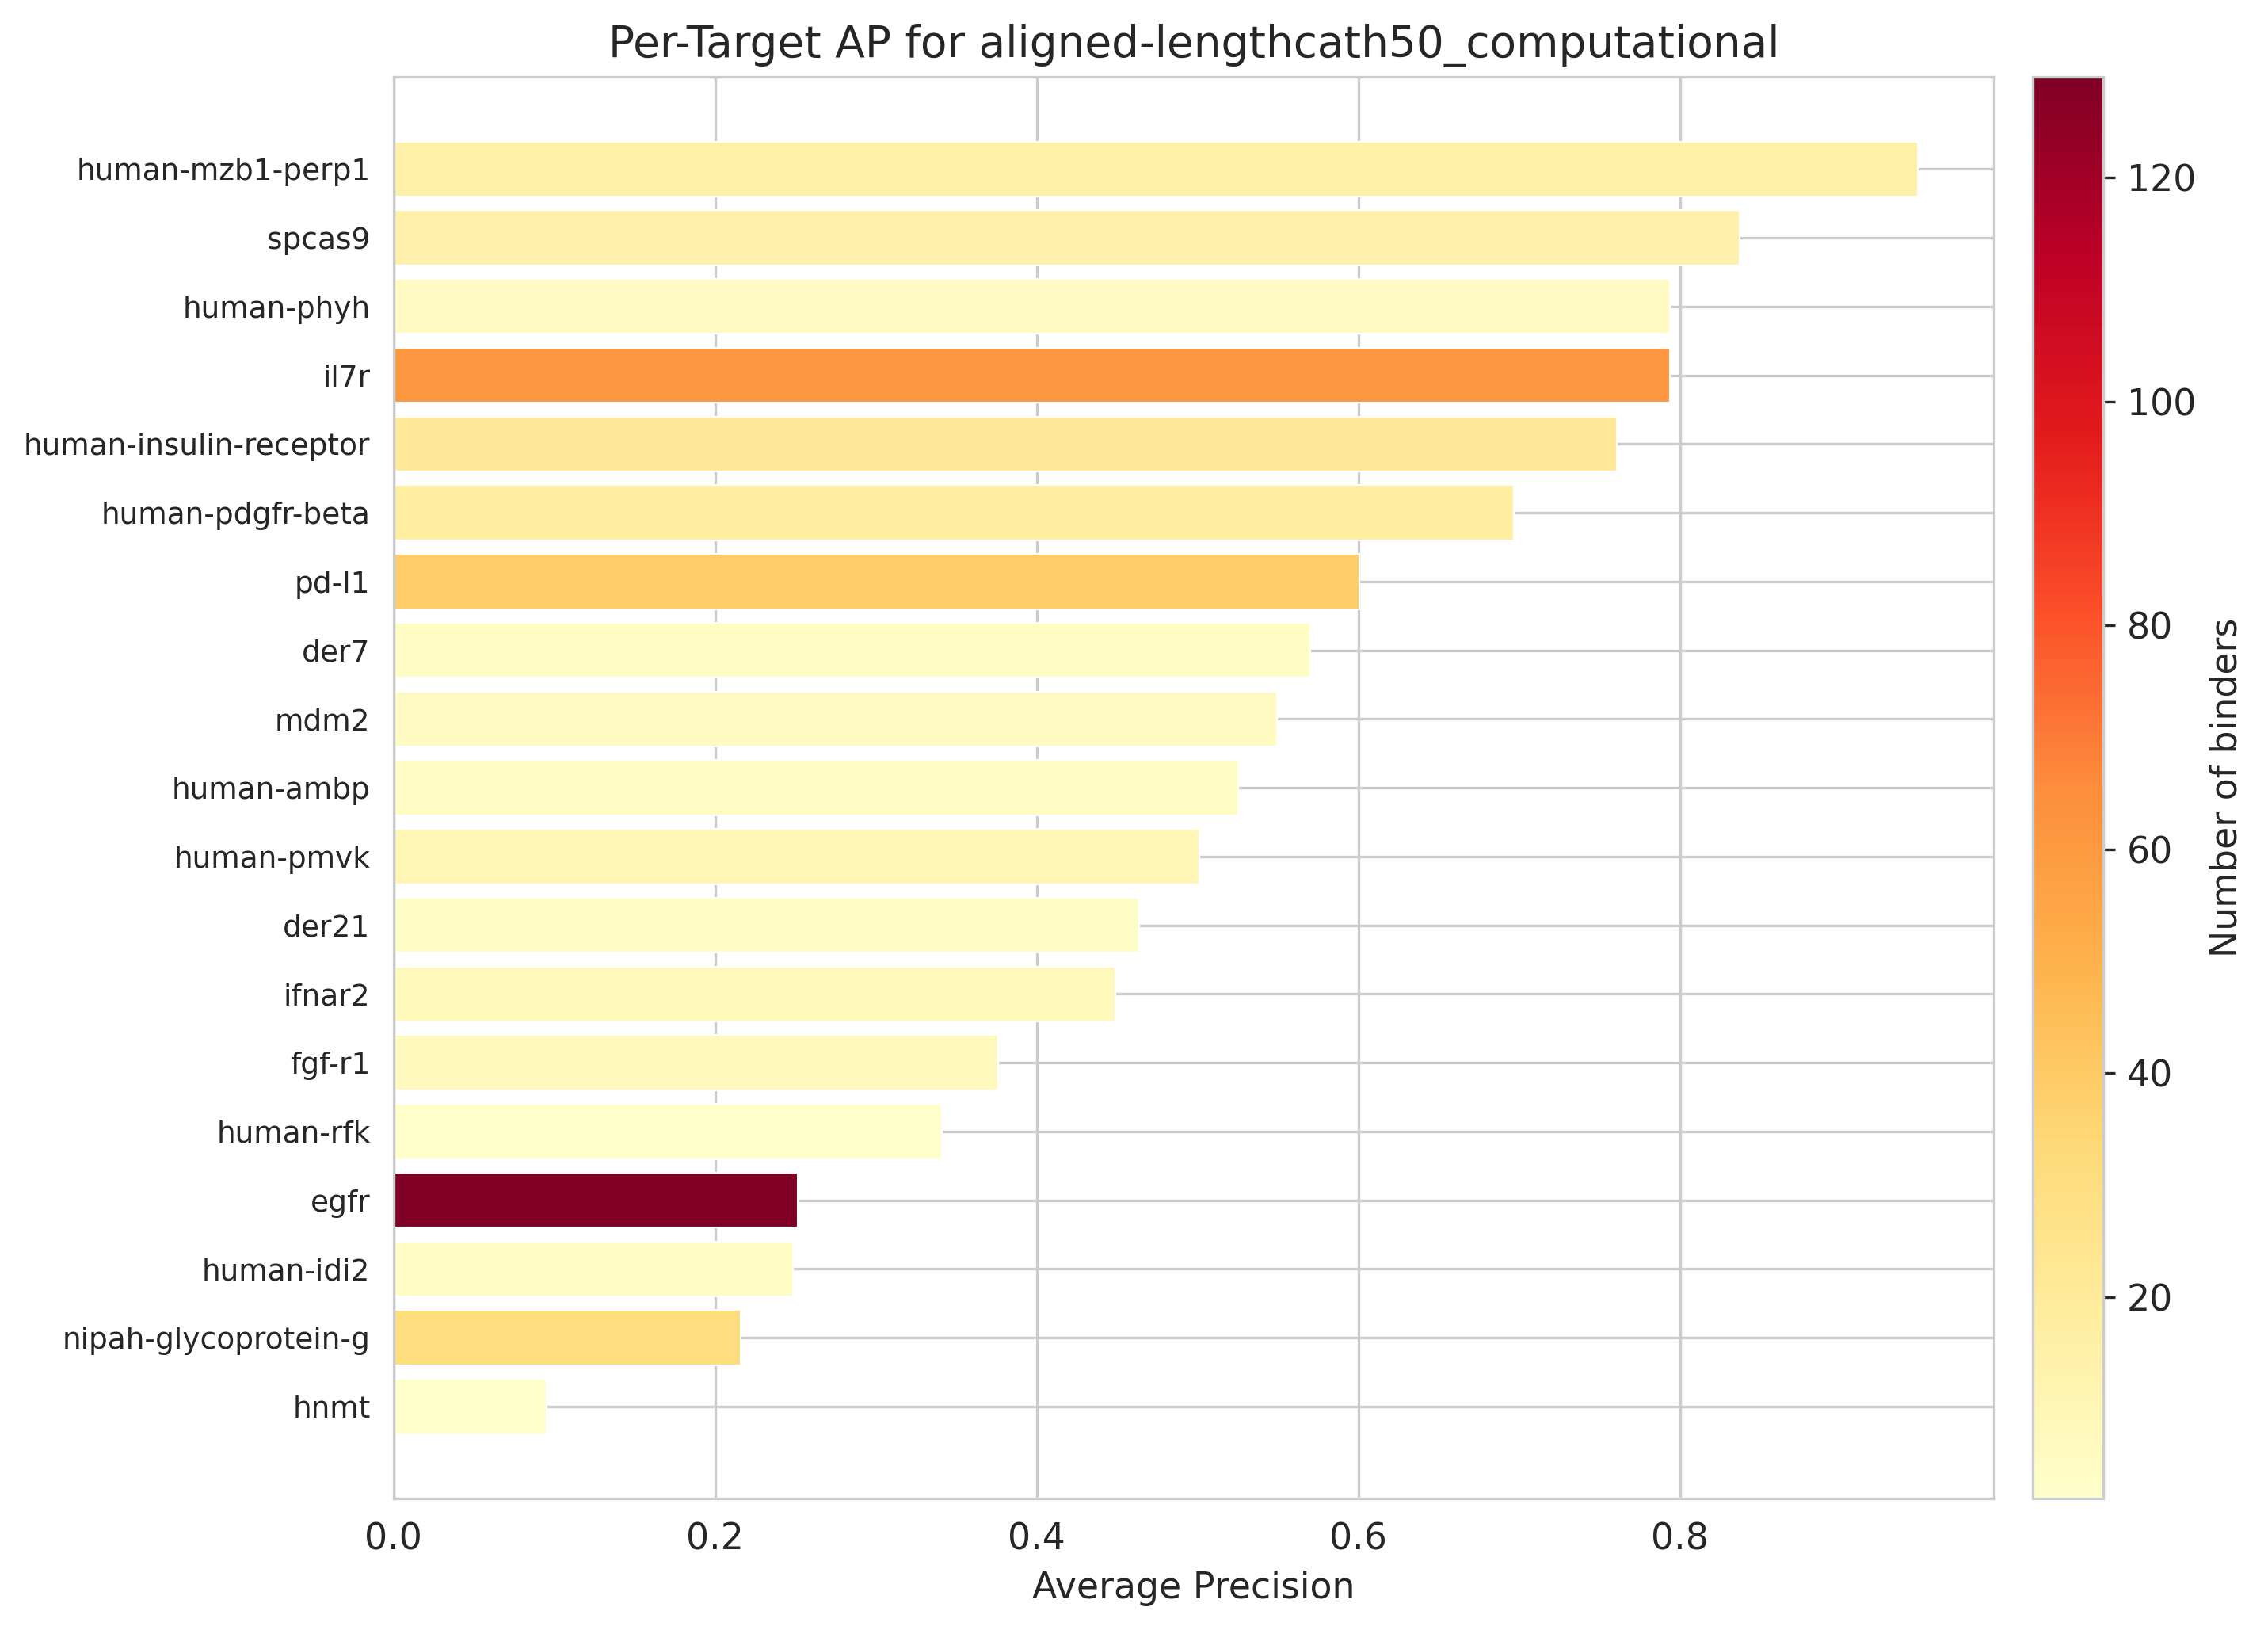
\includegraphics[width=\textwidth]{fig18_per_target_ap.png}
\caption{Average Precision of the best feature for each target. Targets are ordered by AP. Variability across targets is the dominant source of prediction difficulty.}
\label{fig:pertarget}
\end{figure}

Targets with high binding rates (spcas9 at 70\%, il7r at 64\%) tend to be more predictable, while targets with low binding rates and large sample sizes (nipah-glycoprotein-g at 10\%, egfr at 17\%) are harder.
This suggests that target-specific factors---binding site accessibility, conformational flexibility, design strategy quality---dominate over the quality of computational scoring.

\begin{figure}[H]
\centering
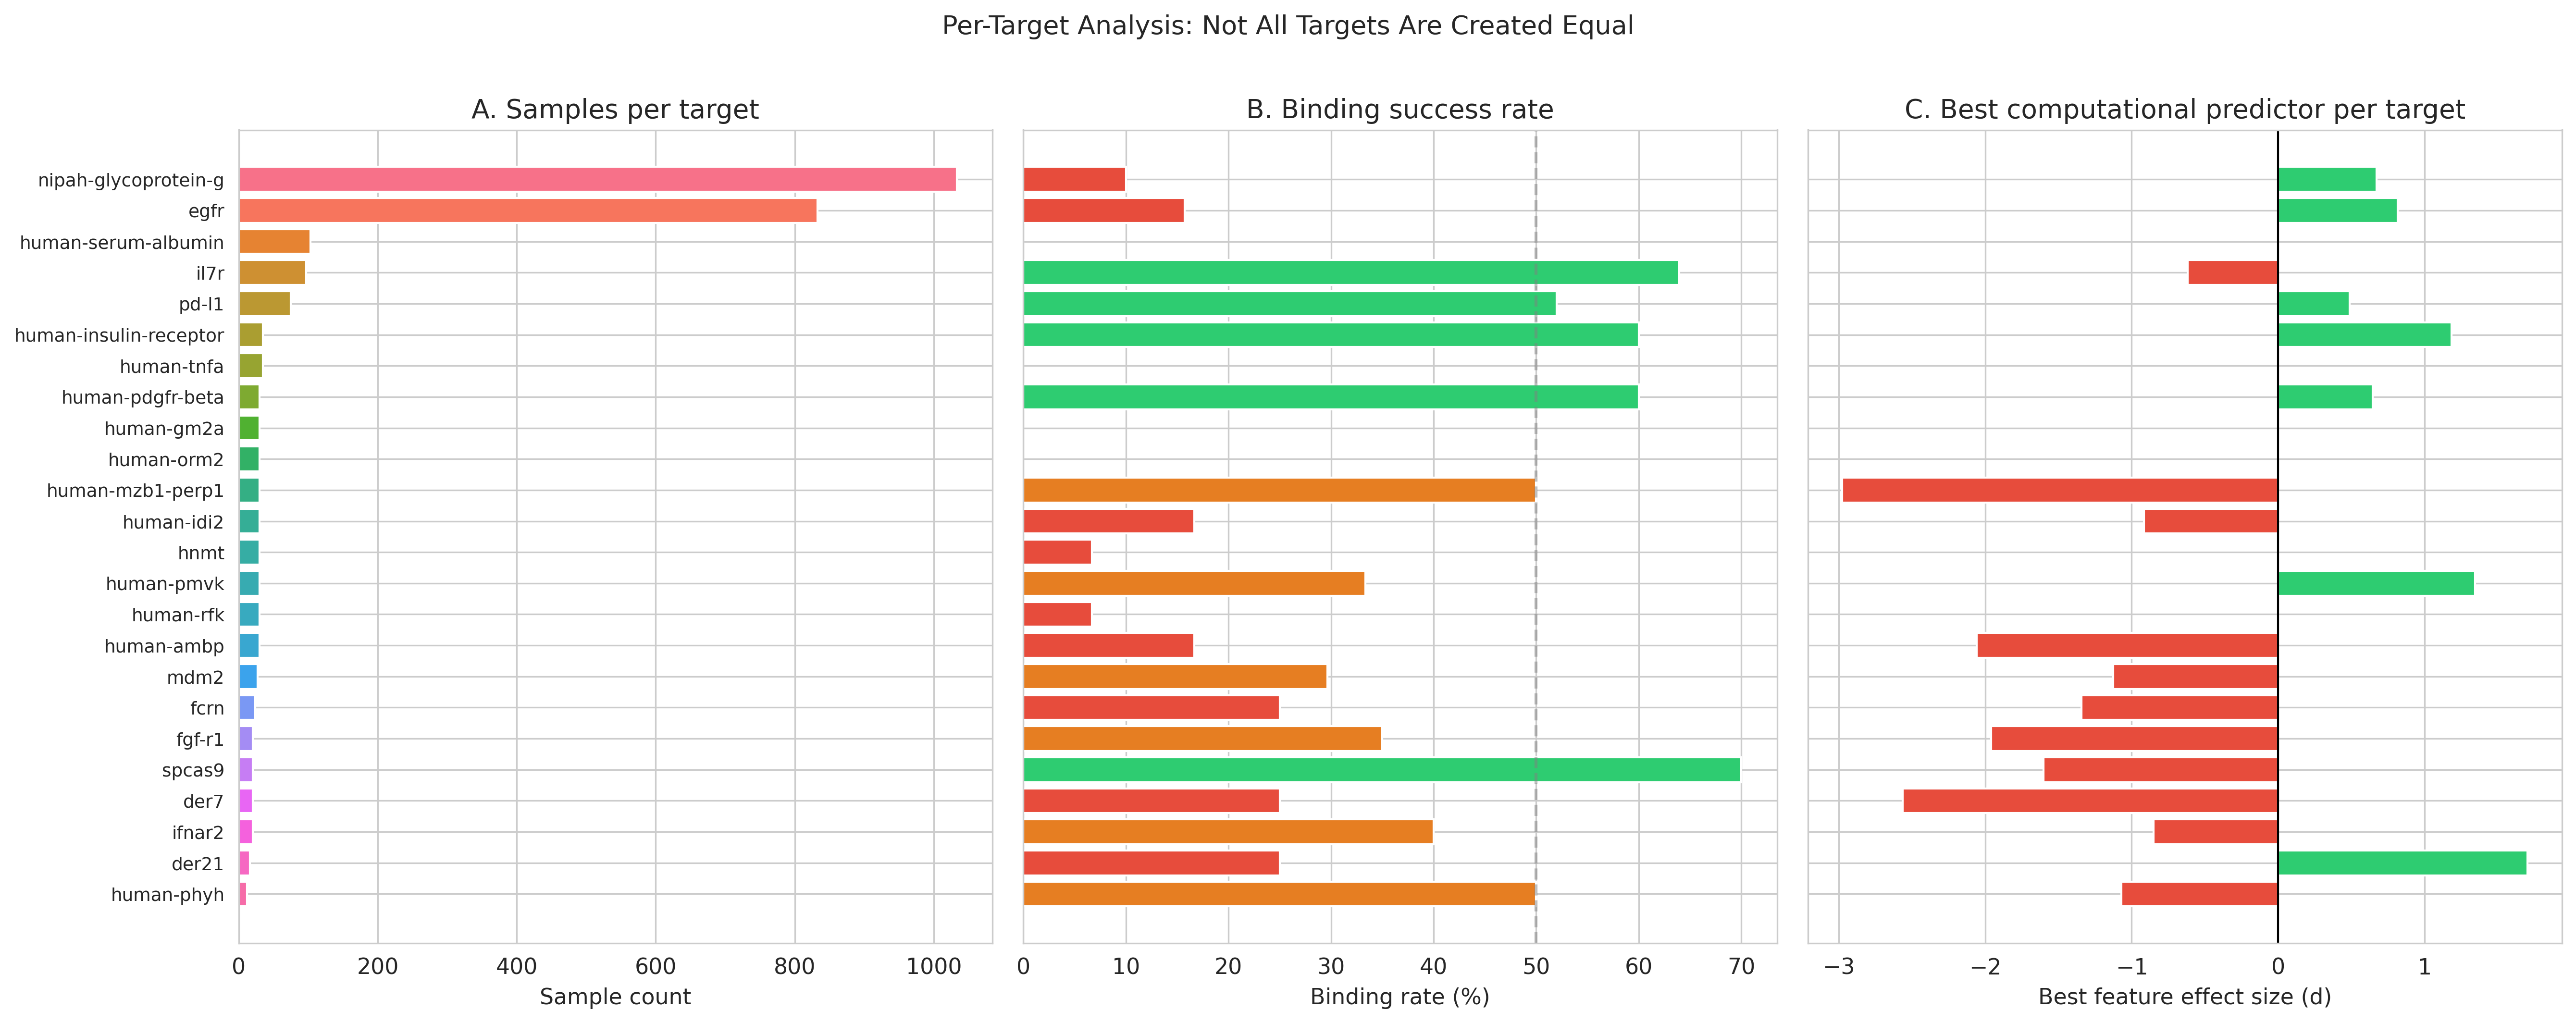
\includegraphics[width=\textwidth]{fig7_per_target.png}
\caption{Per-target comparison showing sample sizes, binding rates, and effect sizes. Targets vary enormously in both tractability and the discriminative power of computational features.}
\label{fig:pertargetdetail}
\end{figure}

\subsection{Binding affinity prediction}

Among confirmed binders, we analyze which features correlate with binding affinity (\pKD).
Sequence identity to the design template is the strongest predictor (Spearman $r = 0.68$, $p = 5.9 \times 10^{-15}$), followed by domain match e-value ($r = -0.55$) and domain match RMSD ($r = -0.50$) (Figure~\ref{fig:pkd}).

\begin{table}[H]
\centering
\caption{Top 10 features correlated with binding affinity (\pKD) among confirmed binders (Spearman rank correlation).}
\label{tab:pkd}
\begin{tabular}{lcrc}
\toprule
Feature & $r_s$ & $p$-value & $n$ \\
\midrule
Sequence identity (template) & 0.677 & $5.9 \times 10^{-15}$ & 102 \\
Domain match e-value (AFDB50) & $-$0.553 & $2.4 \times 10^{-9}$ & 100 \\
Domain match RMSD (AFDB50) & $-$0.496 & $1.6 \times 10^{-7}$ & 100 \\
Domain match TM-score (AFDB50) & 0.491 & $2.1 \times 10^{-7}$ & 100 \\
Domain match aligned-length (AFDB50) & 0.477 & $5.1 \times 10^{-7}$ & 100 \\
\% charged neg.\ & $-$0.300 & $1.8 \times 10^{-10}$ & 435 \\
TM-score (AFDB50) & 0.294 & $1.8 \times 10^{-8}$ & 354 \\
seq.\ identity (PDB100) & 0.287 & $4.0 \times 10^{-8}$ & 352 \\
\bottomrule
\end{tabular}
\end{table}

\begin{figure}[H]
\centering
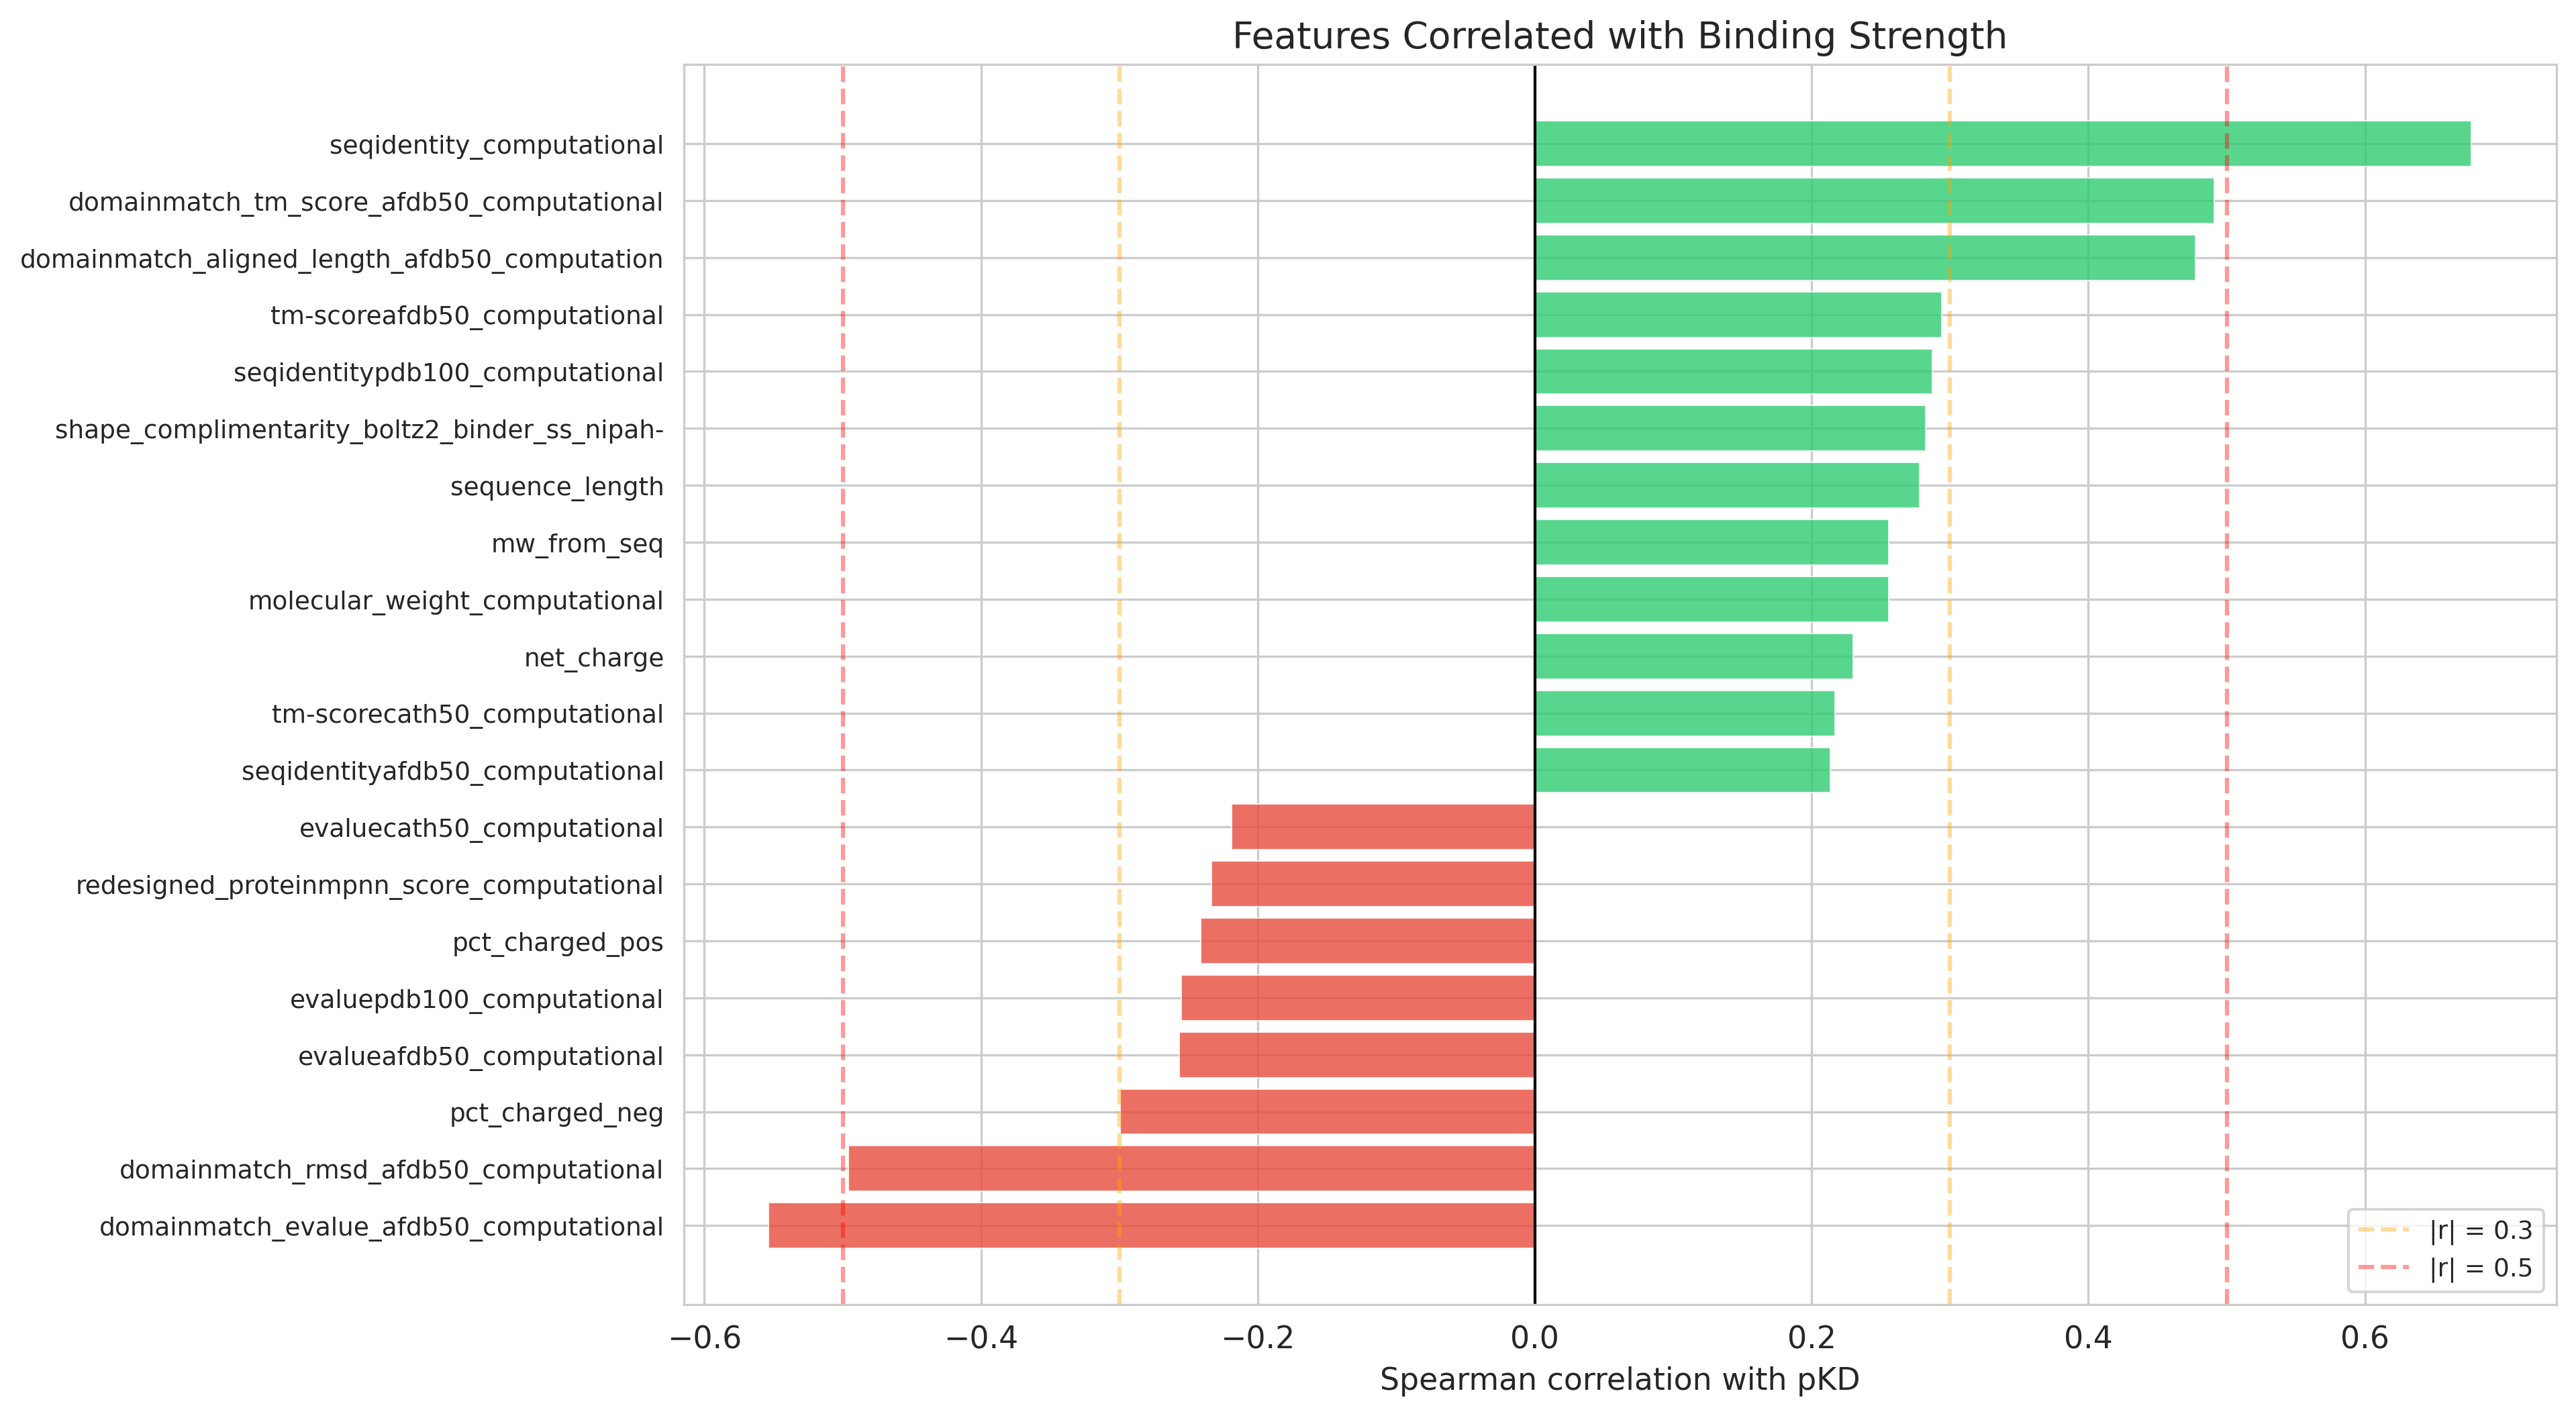
\includegraphics[width=\textwidth]{fig4_pkd_correlations.png}
\caption{Spearman rank correlations between computational features and \pKD\ among confirmed binders. Sequence identity to the design template dominates.}
\label{fig:pkd}
\end{figure}

This finding suggests that designs closely resembling known functional proteins not only bind but bind more tightly, likely because evolutionarily refined binding interfaces have been partially recapitulated.

\subsection{LASSO feature selection}

\subsubsection{Binary binding prediction}

L1-regularized logistic regression selects a single feature: ESMFold pLDDT (coefficient = 0.024).
This extreme sparsity reflects both the high correlation among features and the difficulty of the prediction task at the population level.

\begin{figure}[H]
\centering
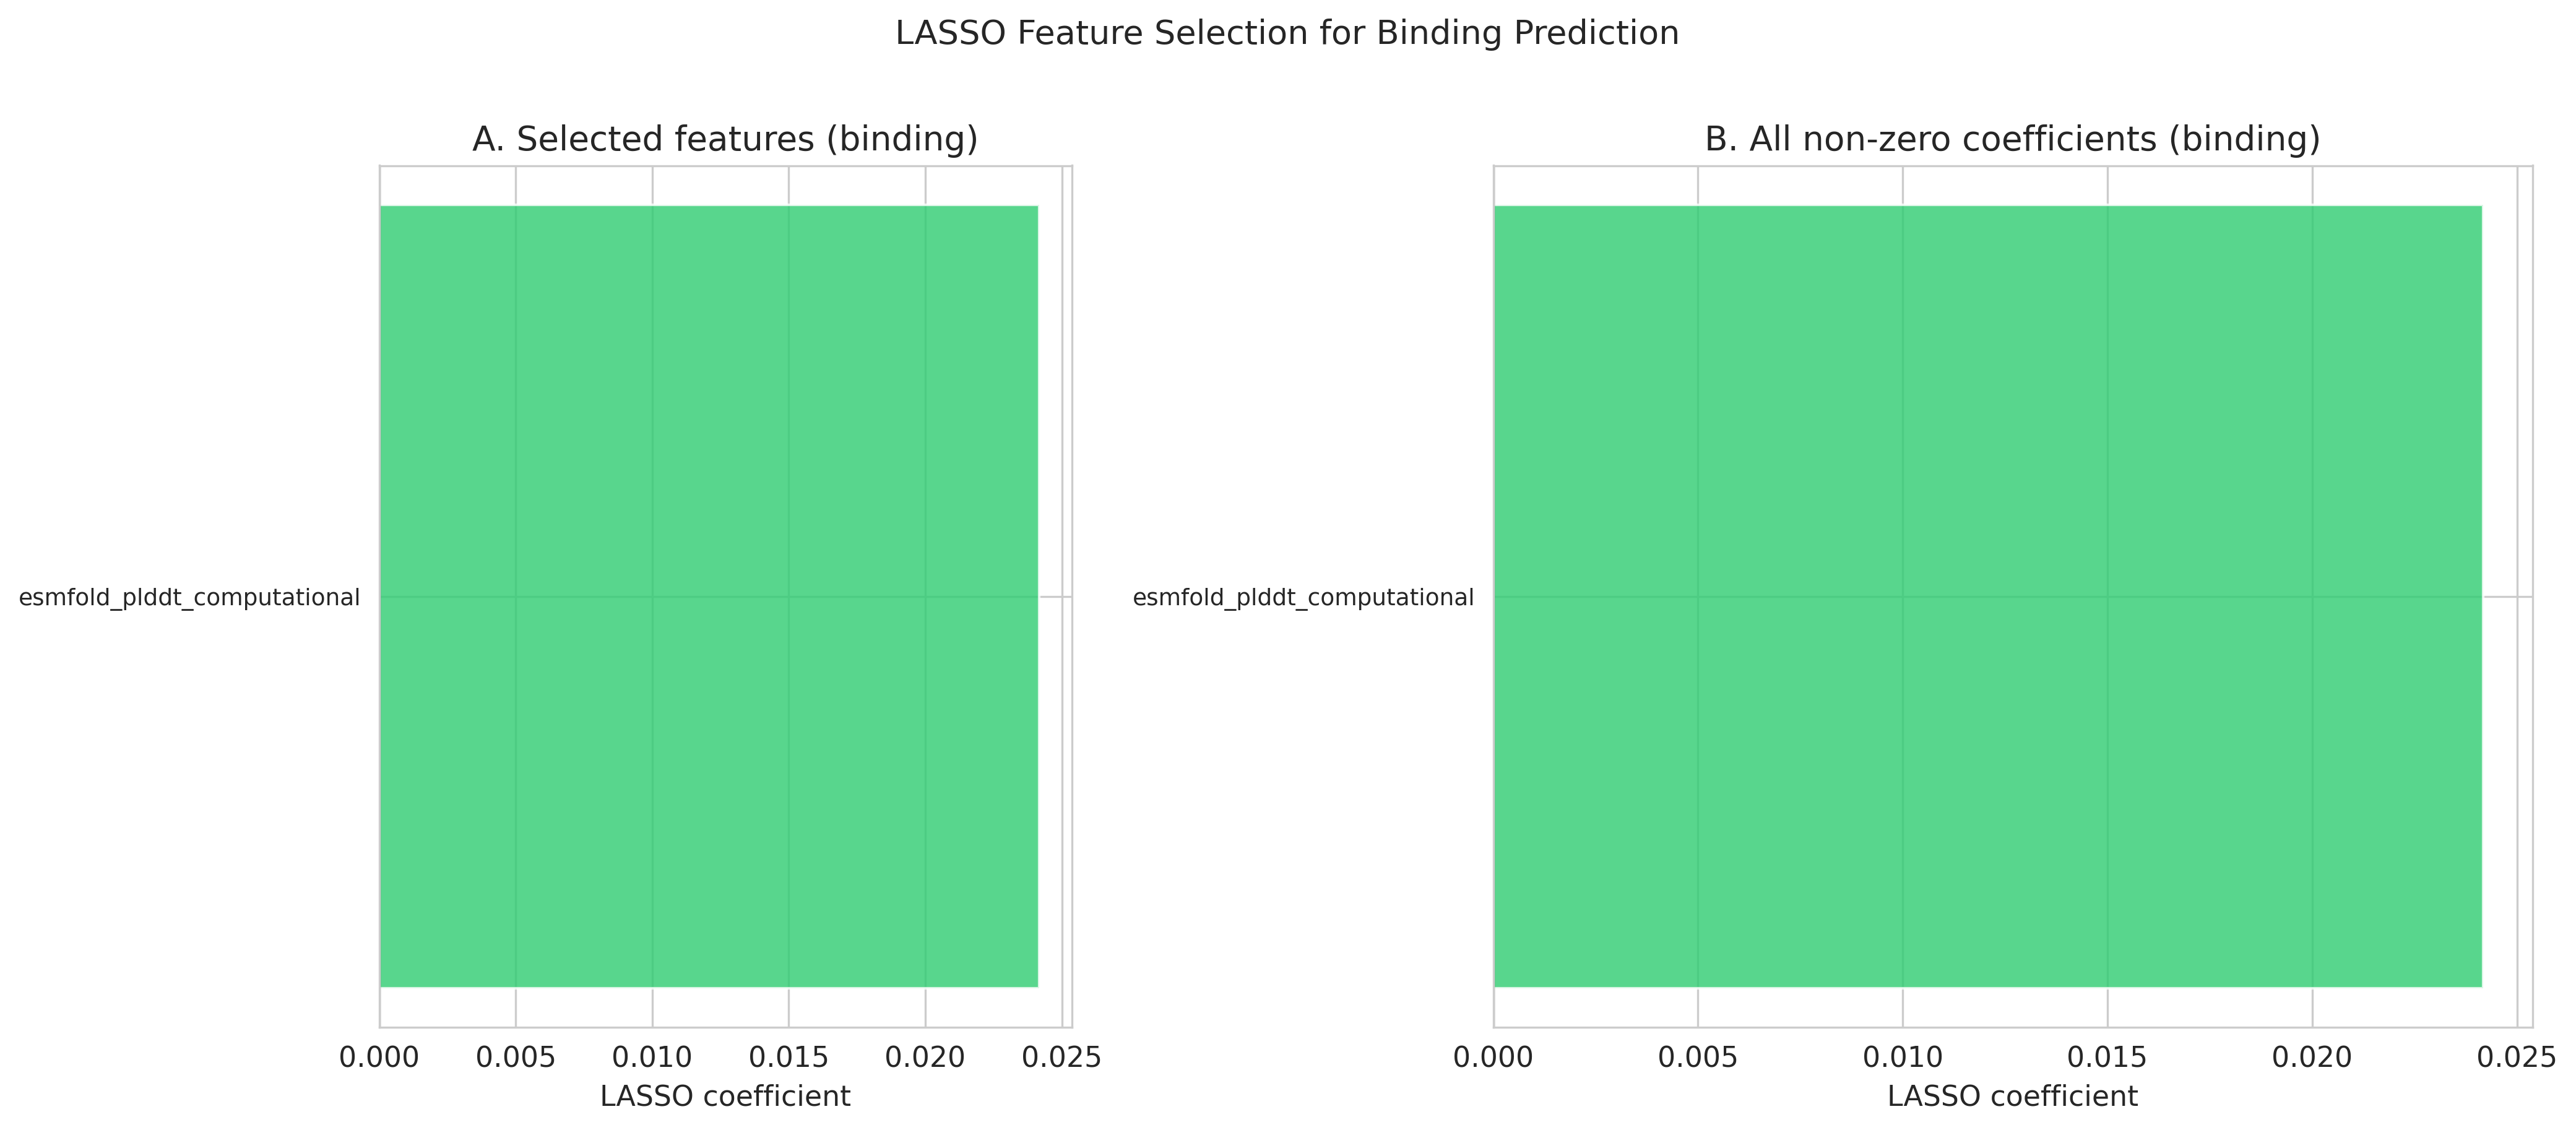
\includegraphics[width=0.85\textwidth]{fig6_lasso_binary.png}
\caption{LASSO coefficients for binary binding prediction. Only ESMFold pLDDT survives L1 regularization.}
\label{fig:lassobinary}
\end{figure}

\subsubsection{Affinity prediction}

For \pKD\ prediction among confirmed binders, LassoCV selects 6 features (Table~\ref{tab:lassopkd}), with sequence length and TM-score (AFDB50) receiving the largest coefficients.

\begin{table}[H]
\centering
\caption{Features selected by LassoCV for \pKD\ prediction, with standardized coefficients.}
\label{tab:lassopkd}
\begin{tabular}{lc}
\toprule
Feature & Coefficient \\
\midrule
Sequence length & 0.188 \\
TM-score (AFDB50) & 0.085 \\
\% charged neg.\ & $-$0.067 \\
TED confidence & 0.022 \\
TM-score (CATH50) & 0.008 \\
Net charge & 0.004 \\
\bottomrule
\end{tabular}
\end{table}

\begin{figure}[H]
\centering
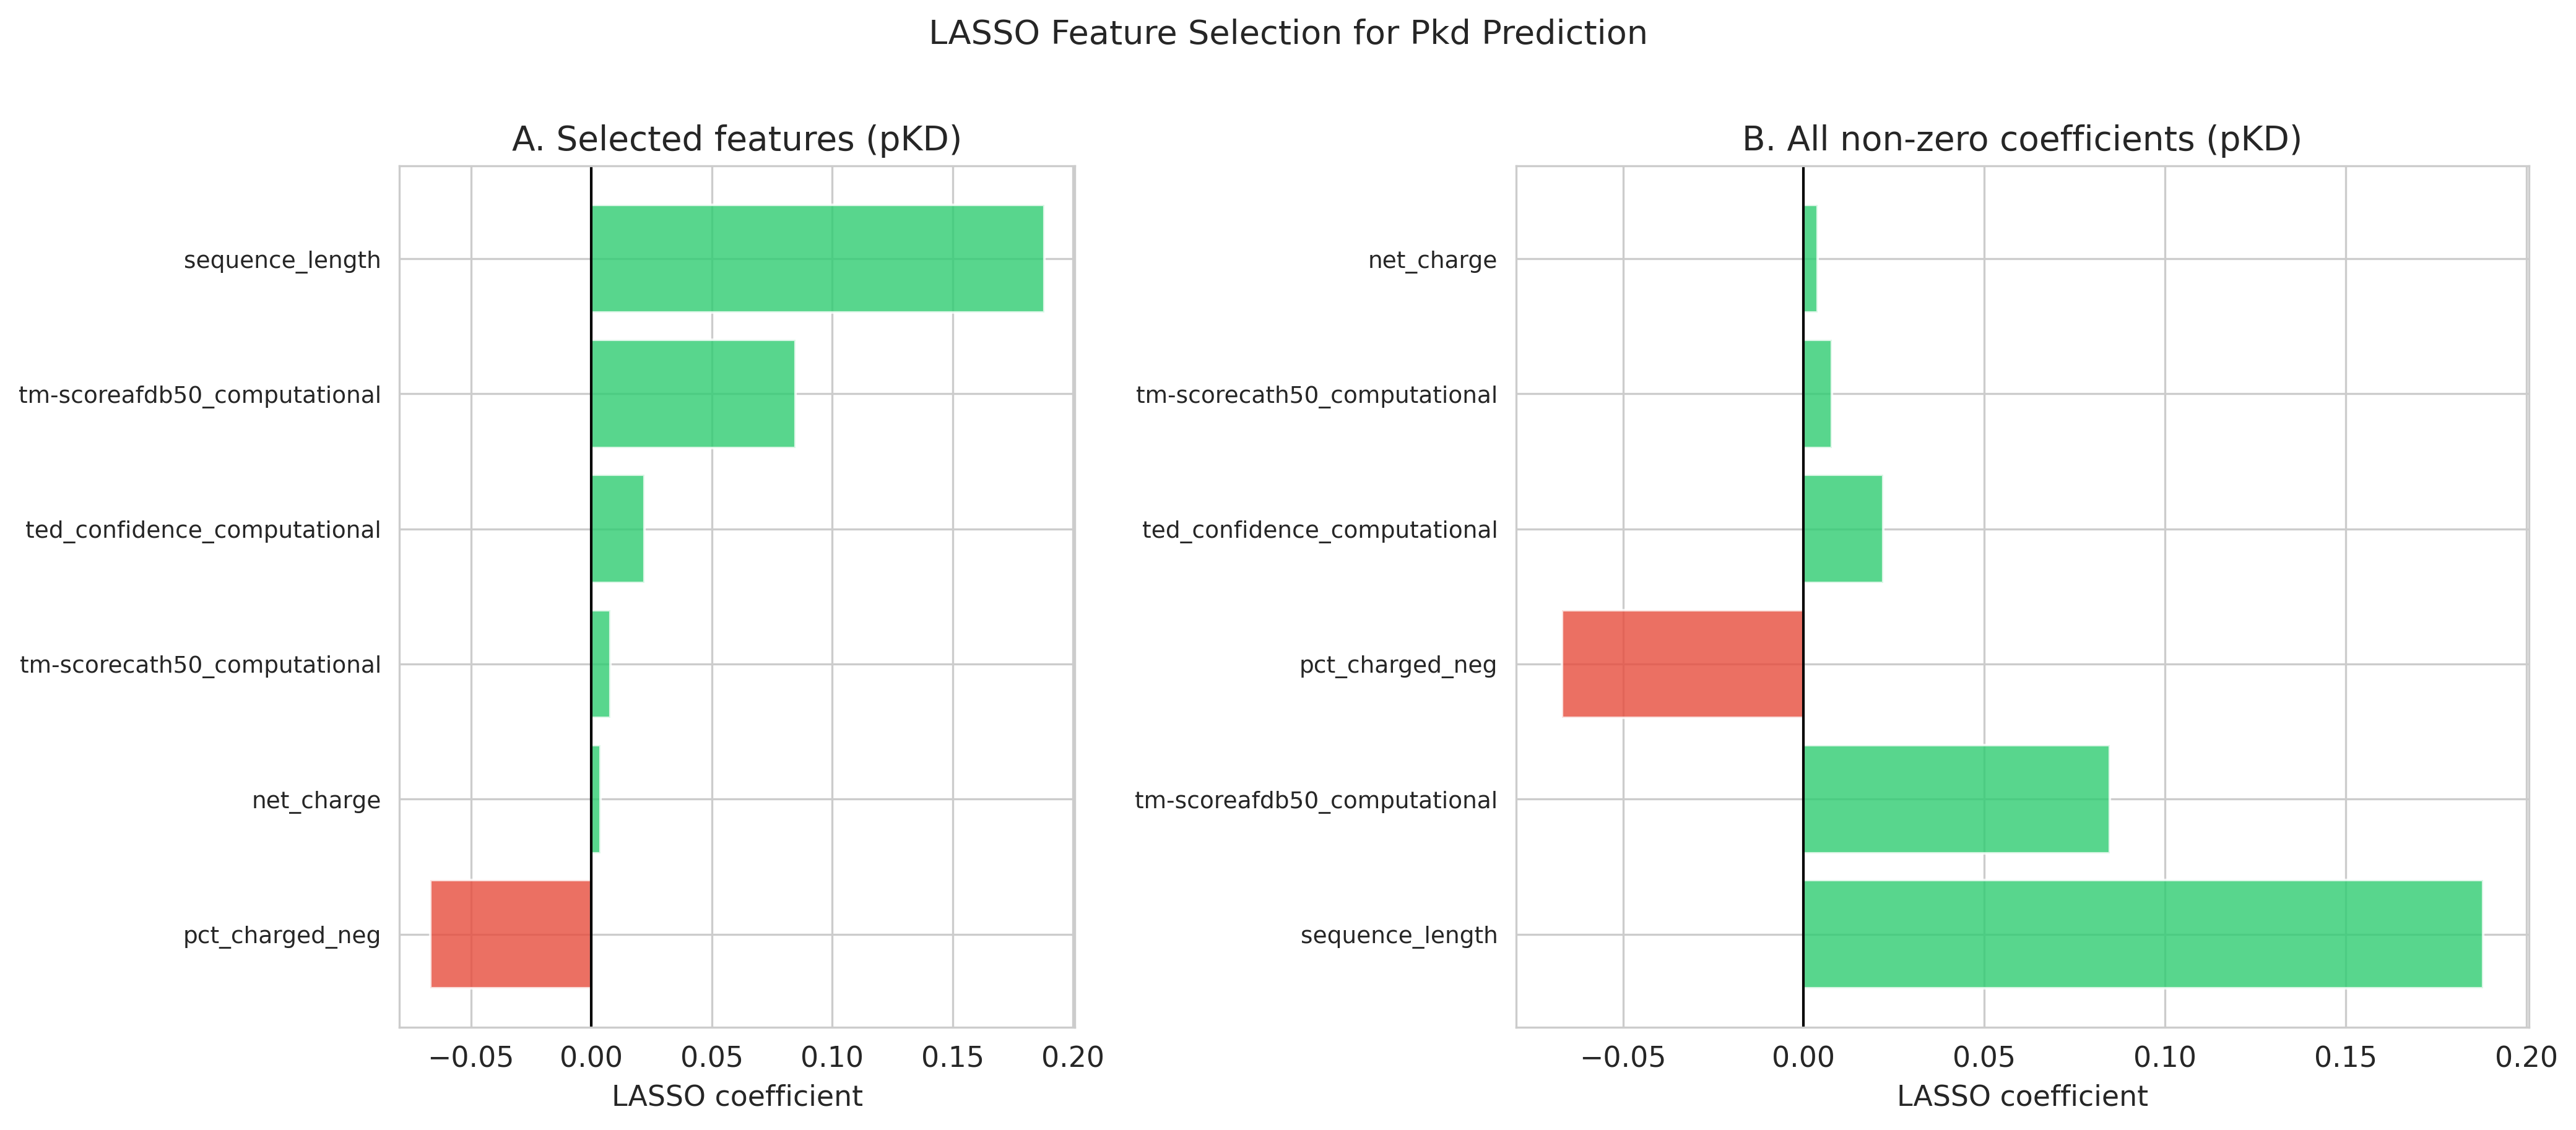
\includegraphics[width=0.85\textwidth]{fig6_lasso_pkd.png}
\caption{LASSO coefficients for \pKD\ prediction. Six features are selected, with sequence length contributing most.}
\label{fig:lassopkd}
\end{figure}

\subsection{Greedy forward selection}

Greedy selection with LOGO-CV converges at 2 features (Figure~\ref{fig:greedy}):

\begin{enumerate}
    \item Positive charge fraction (AP = 0.573 after step 1)
    \item TM-score from PDB100 (AP = 0.605 after step 2)
\end{enumerate}

\begin{figure}[H]
\centering
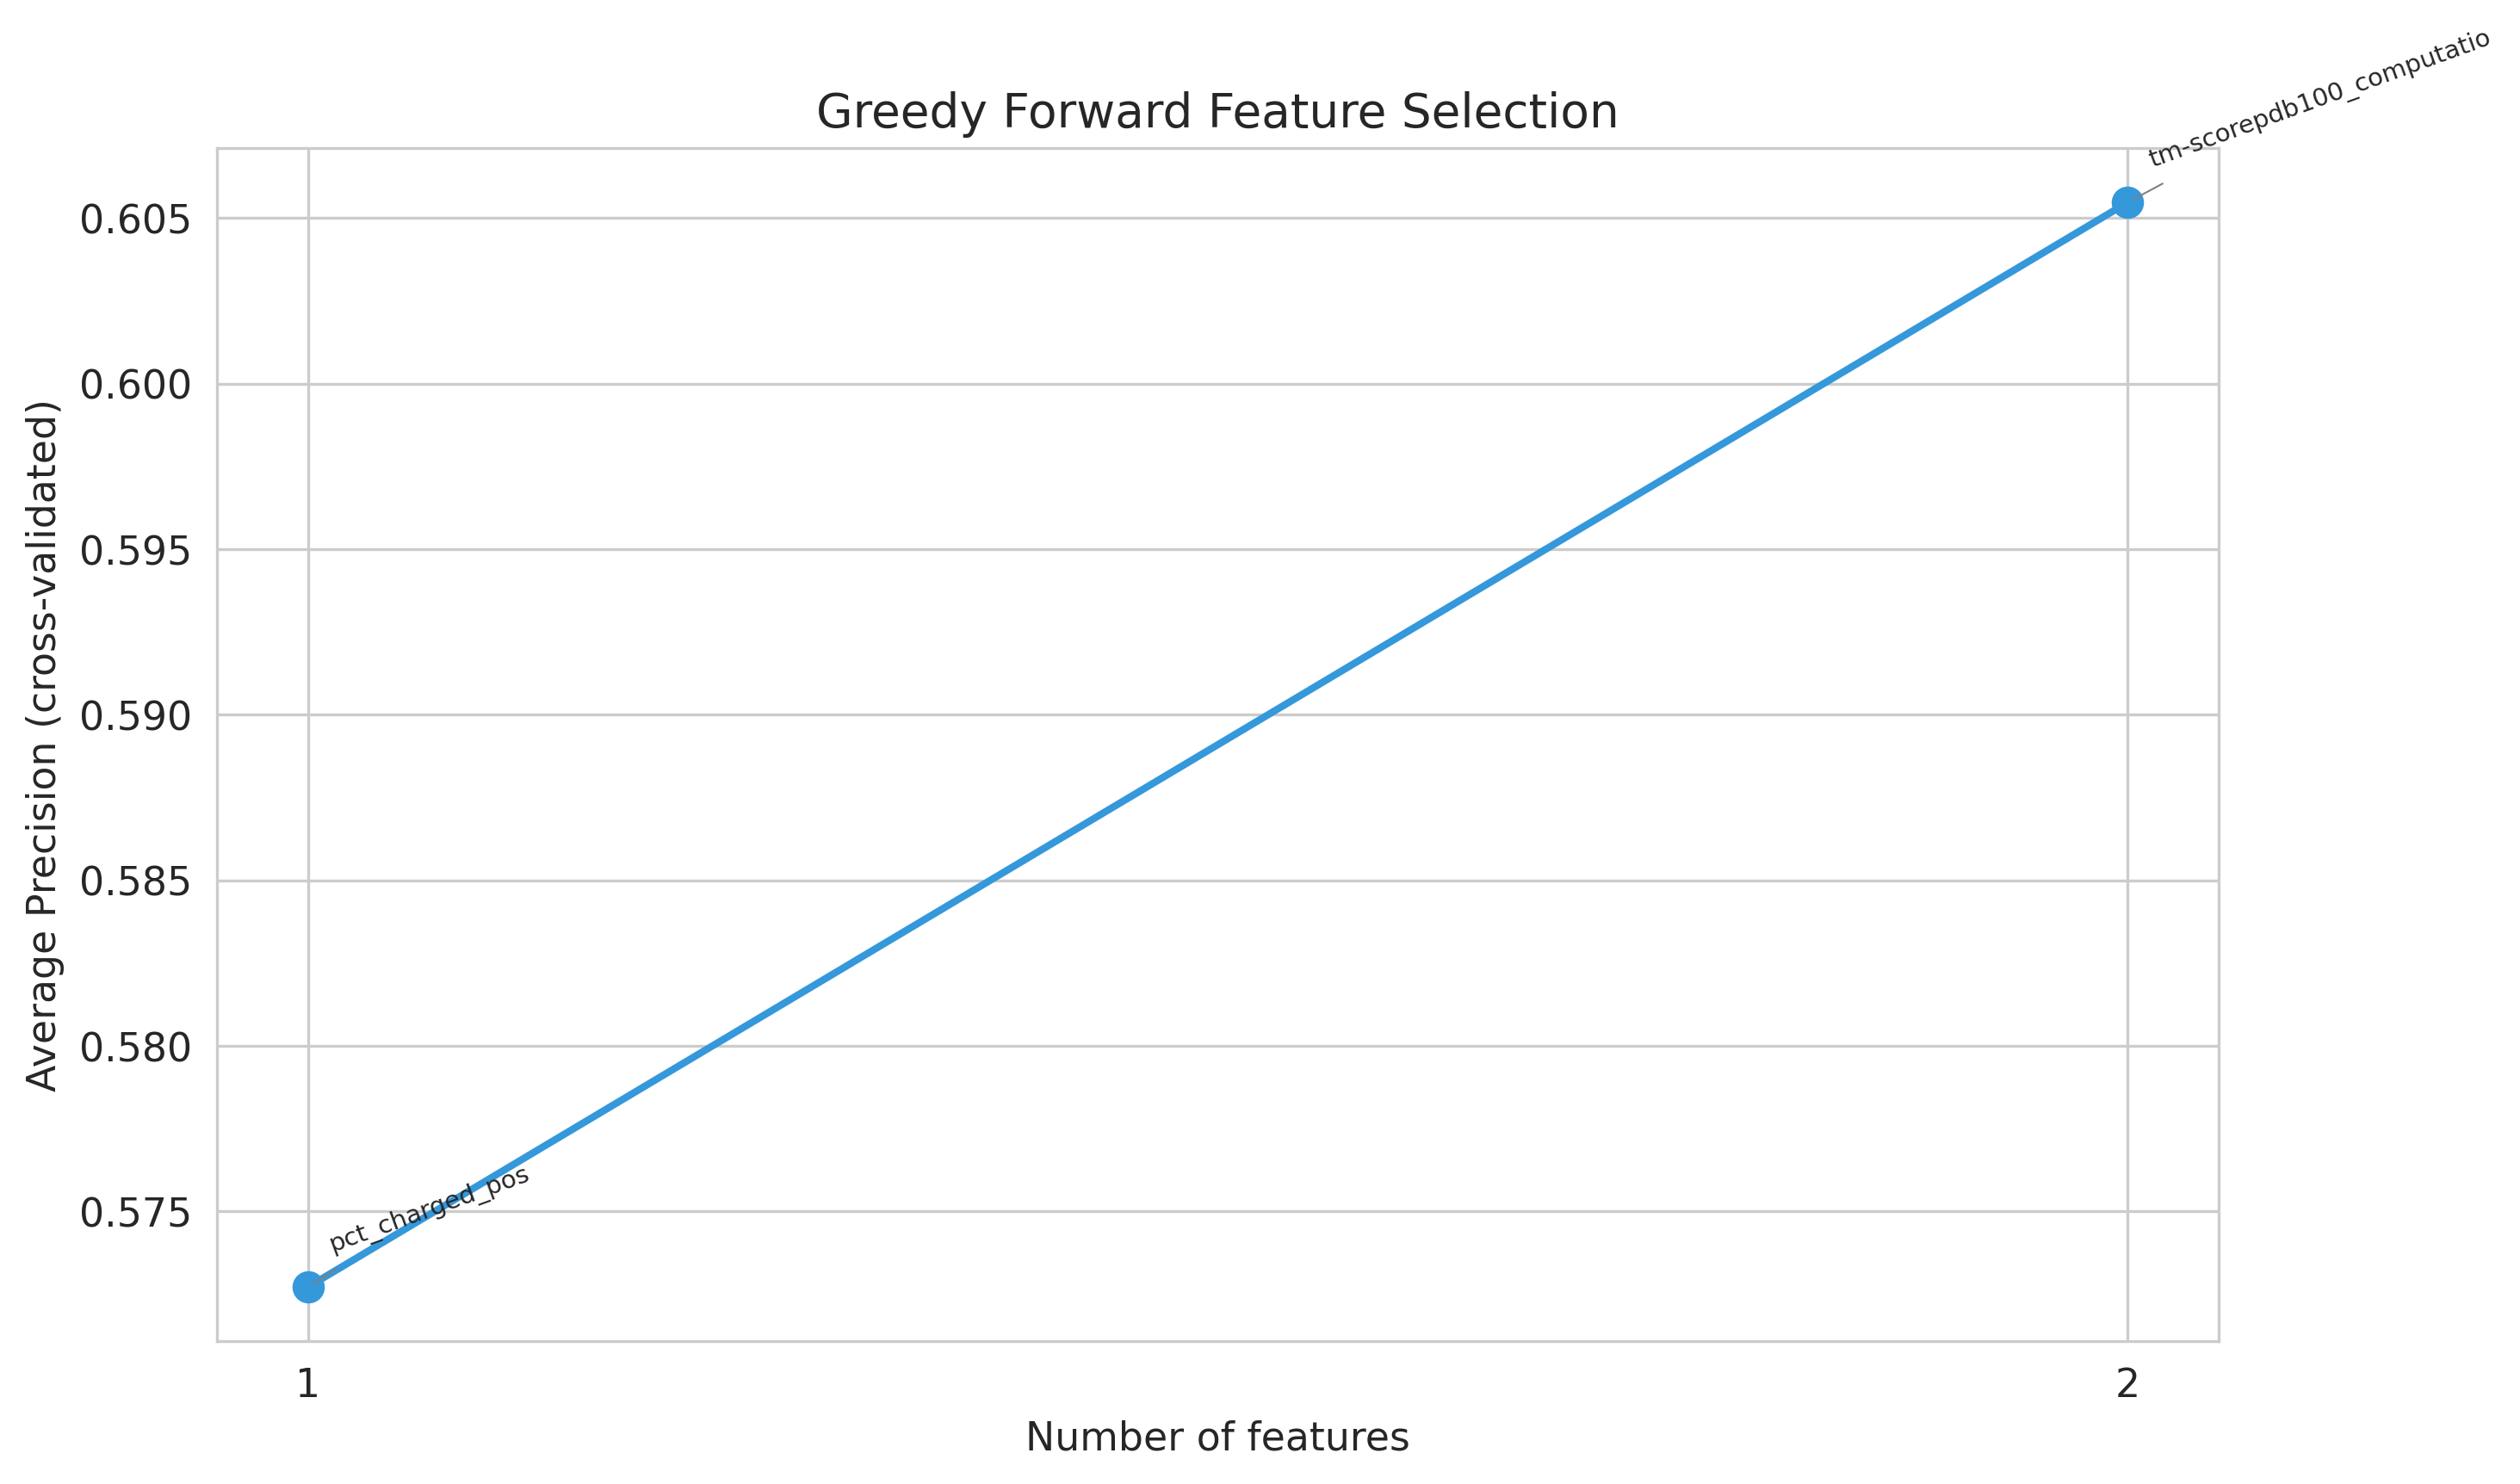
\includegraphics[width=0.85\textwidth]{fig11_greedy_progress.png}
\caption{Greedy forward selection with LOGO-CV. AP plateaus after 2 features, consistent with Overath et al.'s finding that 2--5 features suffice.}
\label{fig:greedy}
\end{figure}

This rapid convergence is consistent with Overath et al., who found that 2--5 features are optimal before additional features introduce noise from cross-target heterogeneity.
The selected pair---a physicochemical property (charge fraction) and a structural metric (TM-score)---aligns with the interaction feature analysis, confirming that these two feature classes provide complementary predictive information.

\subsection{Model performance}

The final model (L1 logistic regression on LASSO-selected features) achieves:

\begin{table}[H]
\centering
\caption{Final model performance metrics.}
\label{tab:model}
\begin{tabular}{lc}
\toprule
Metric & Value \\
\midrule
Average Precision & 0.211 \\
ROC-AUC & 0.596 \\
F1 score & 0.345 \\
Precision & 0.216 \\
Recall & 0.866 \\
Optimal threshold & 0.474 \\
\bottomrule
\end{tabular}
\end{table}

The high recall (0.87) at the cost of low precision (0.22) reflects the threshold optimized for F1 on this imbalanced dataset.
The AP of 0.211 is above the baseline rate of 0.179, indicating the model is learning useful signal, but the improvement is modest---consistent with the inherent difficulty of cross-target binding prediction.

\begin{figure}[H]
\centering
\begin{subfigure}[t]{0.48\textwidth}
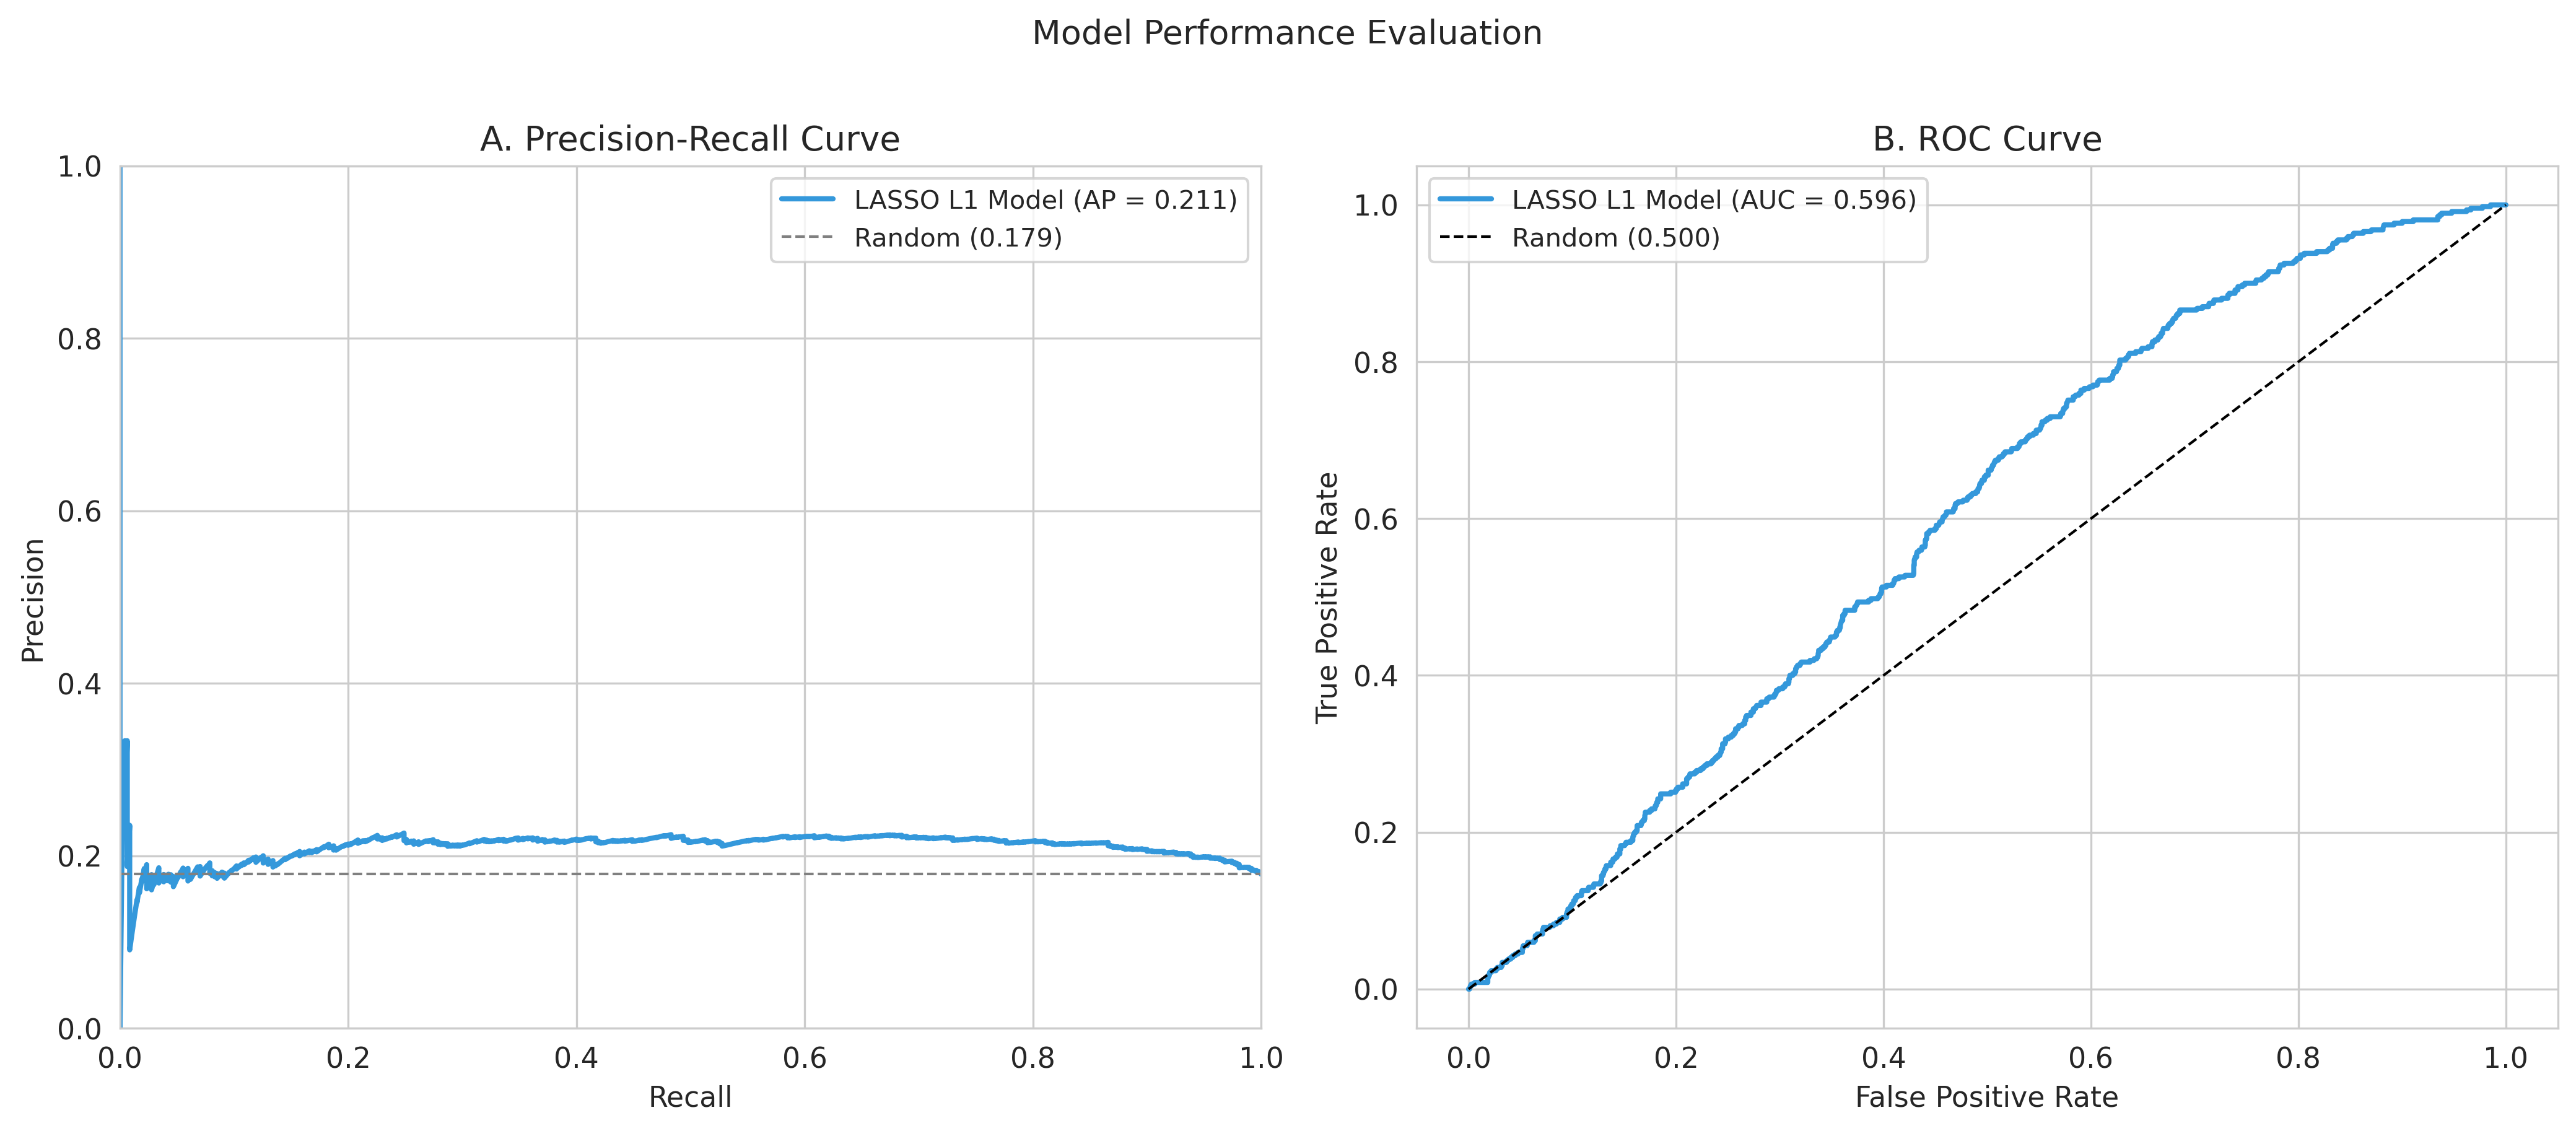
\includegraphics[width=\textwidth]{fig12_pr_roc.png}
\caption{Precision-Recall and ROC curves.}
\end{subfigure}
\hfill
\begin{subfigure}[t]{0.48\textwidth}
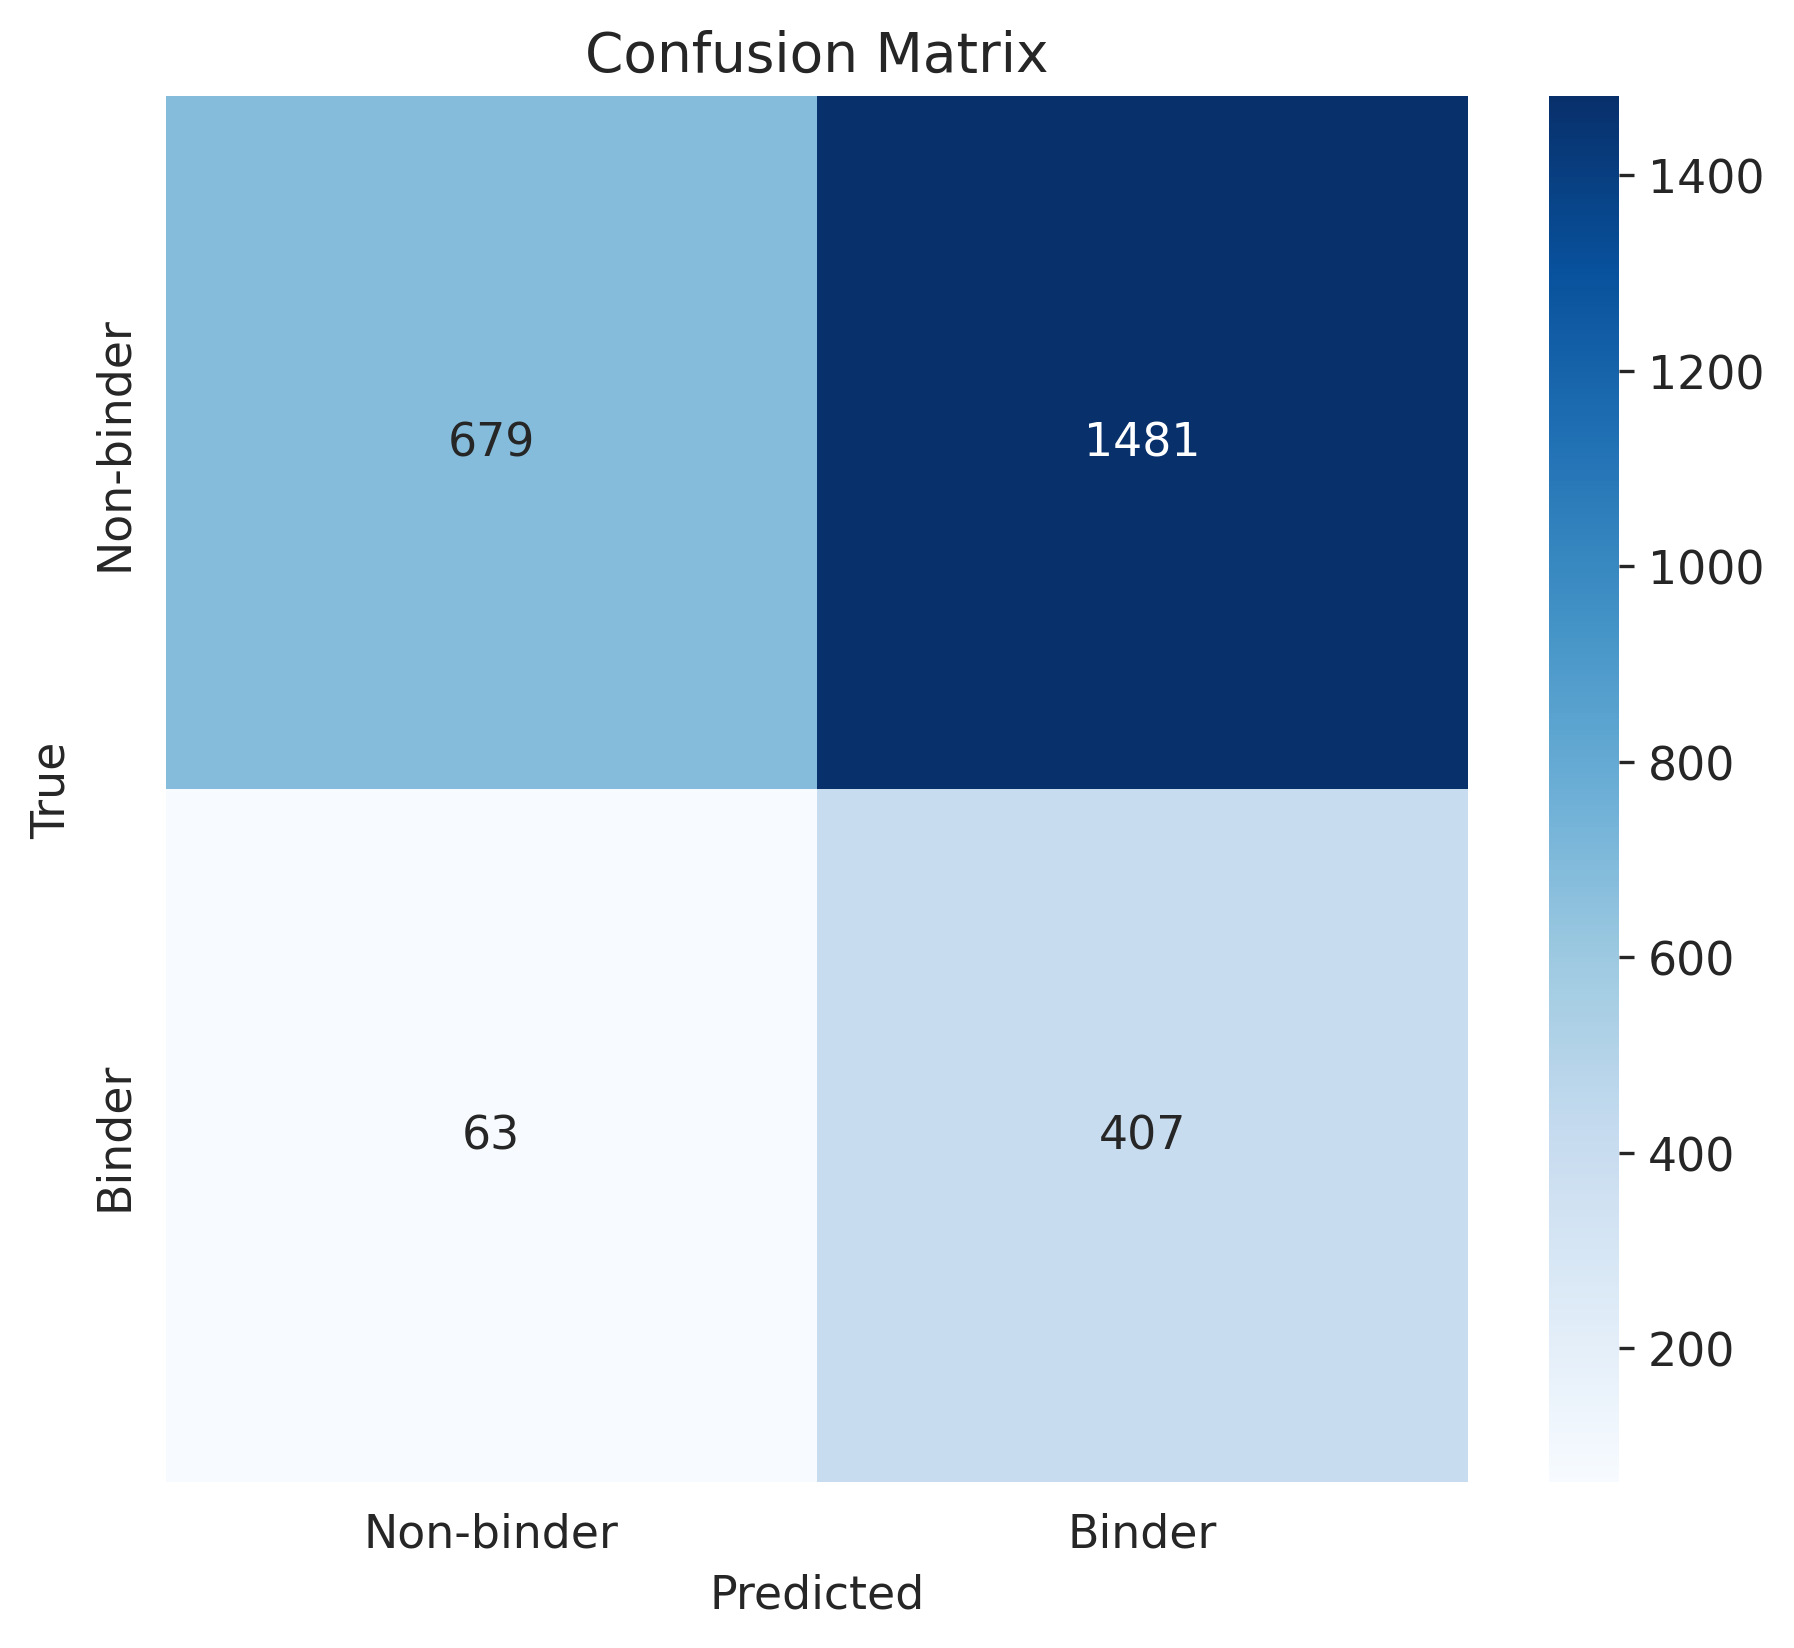
\includegraphics[width=\textwidth]{fig14_confusion.png}
\caption{Confusion matrix at optimal threshold.}
\end{subfigure}
\caption{Model evaluation. (a) The PR curve shows modest separation from the baseline. (b) The confusion matrix at the F1-optimal threshold shows high recall with many false positives.}
\label{fig:model}
\end{figure}

\subsection{Enrichment analysis}

For practical experimental prioritization, enrichment curves (Figure~\ref{fig:enrichment}) show that ranking designs by model score and selecting the top-$k$ yields precision of approximately 50\% in the top 10 designs, dropping to approximately 20\% in the top 100.
This represents a 3--5$\times$ enrichment over random selection, which is practically useful for reducing experimental costs.

\begin{figure}[H]
\centering
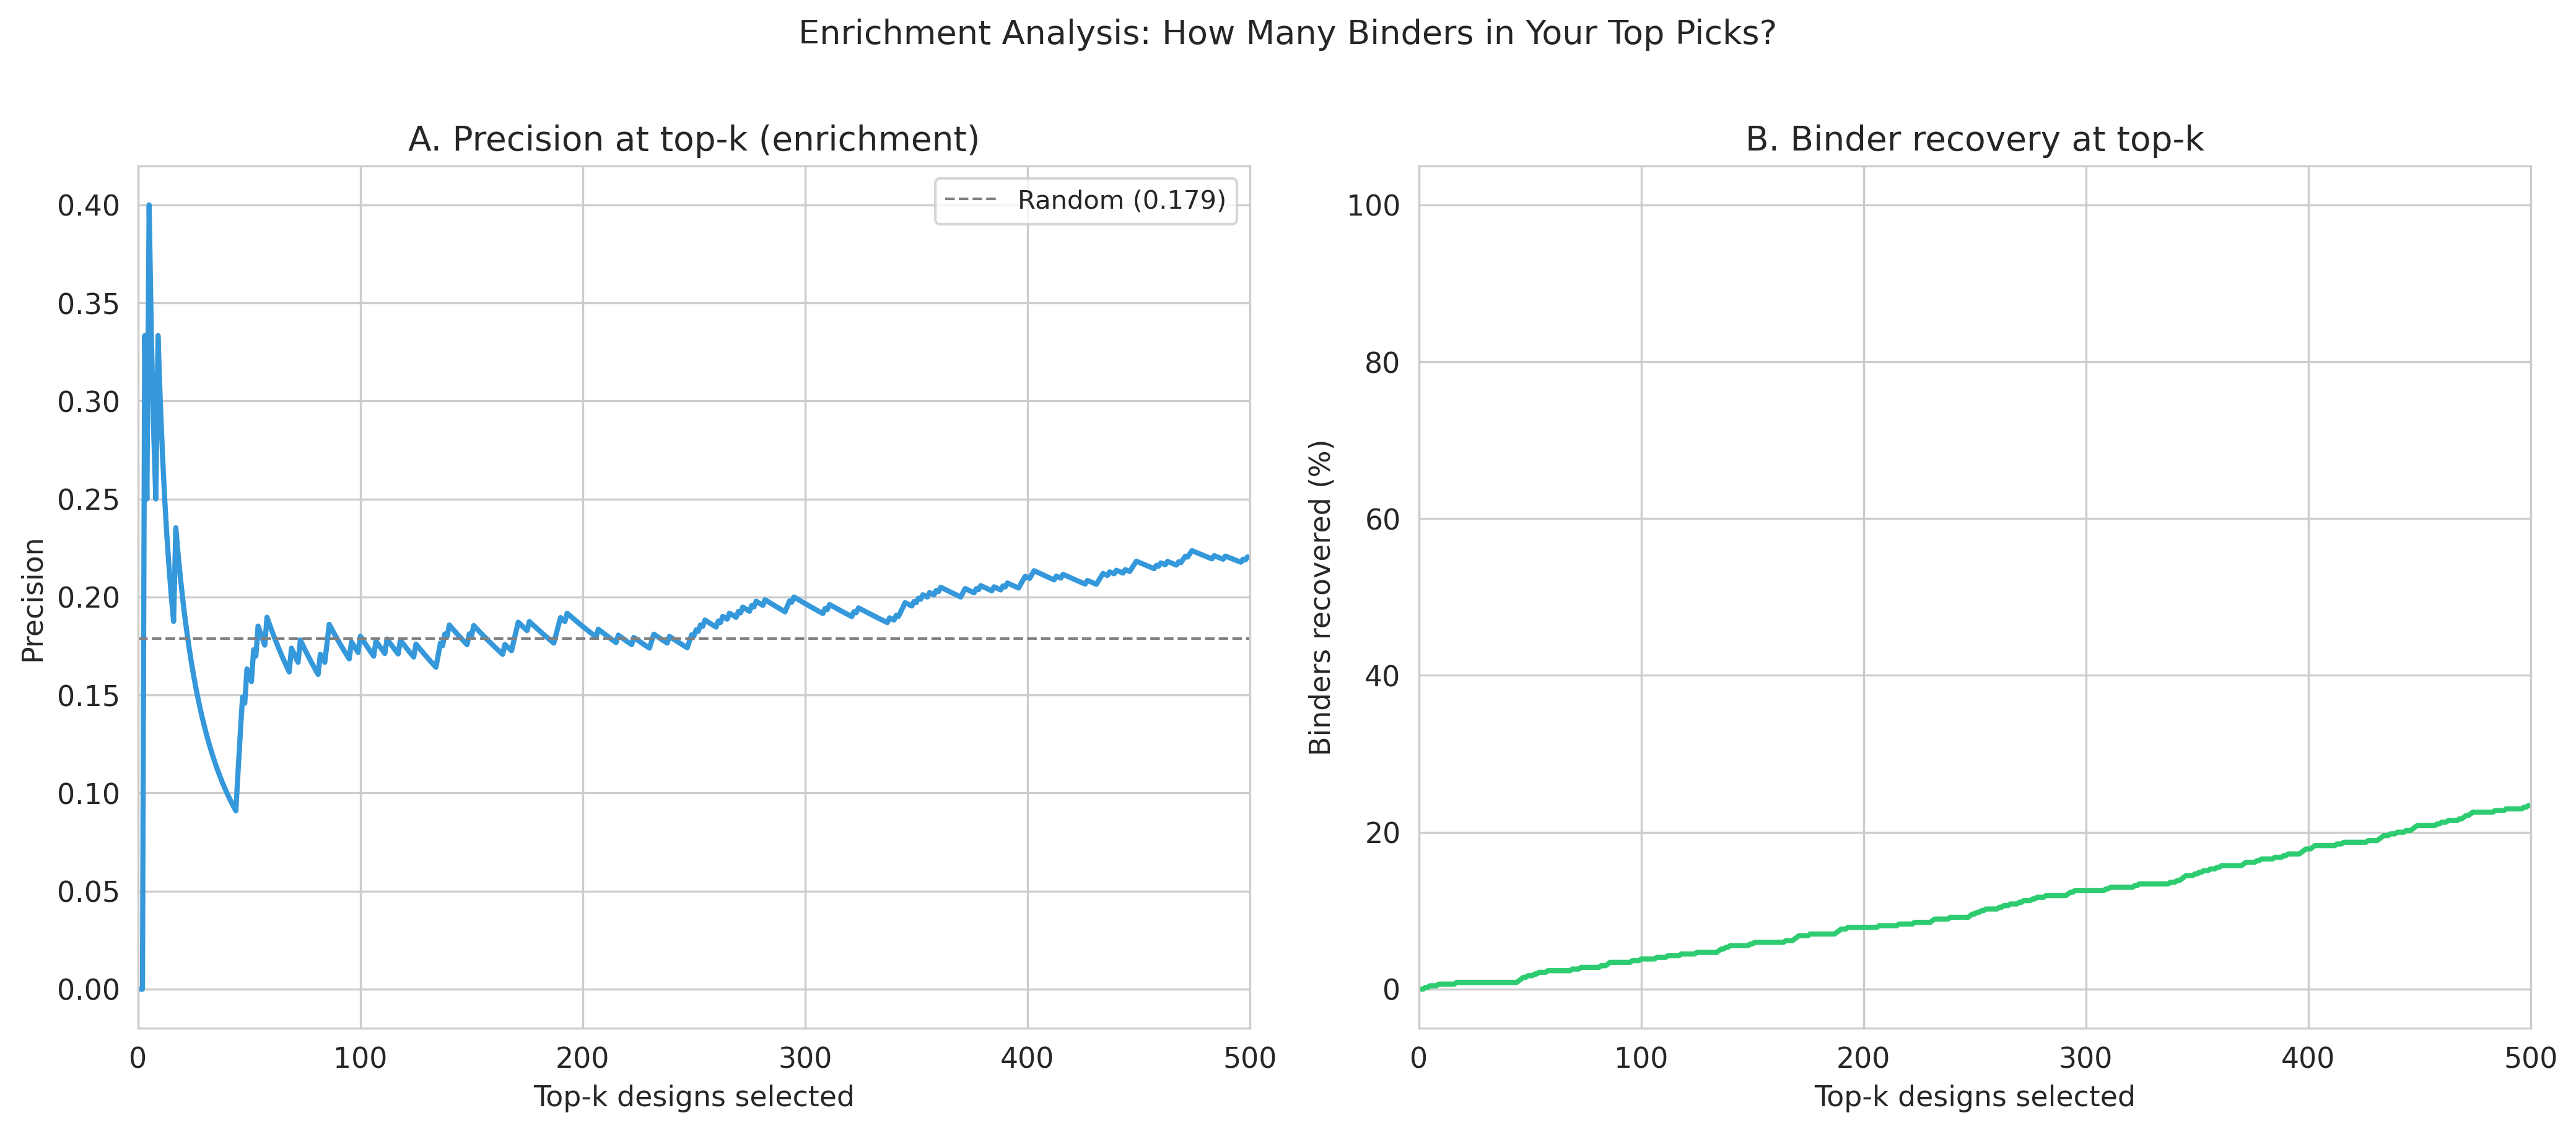
\includegraphics[width=0.85\textwidth]{fig15_enrichment.png}
\caption{Enrichment curves showing precision at top-$k$ (left) and cumulative binder recovery (right). The model enriches binders 3--5$\times$ over random selection in the top 10--50 designs.}
\label{fig:enrichment}
\end{figure}

\subsection{Feature consistency across targets}

We assess which features consistently appear in the top 5 predictors across all 24 targets (Table~\ref{tab:consistency}).
Negative charge fraction is the most consistent, appearing in the top 5 for 6 targets, followed by hydrophobicity, ProteinMPNN redesign score, and GRAVY index (5 targets each).

\begin{table}[H]
\centering
\caption{Feature consistency: number of targets for which each feature appears in the top 5 by AP.}
\label{tab:consistency}
\begin{tabular}{lc}
\toprule
Feature & Targets (out of 24) \\
\midrule
\% charged neg.\ & 6 \\
\% hydrophobic & 5 \\
Redesigned ProteinMPNN score & 5 \\
GRAVY index & 5 \\
seq.\ identity (AFDB50) & 4 \\
MW from sequence & 4 \\
ProteinMPNN seq.\ recovery & 4 \\
Net charge & 4 \\
Charge density & 4 \\
TM-score (CATH50) & 4 \\
Molecular weight & 4 \\
\bottomrule
\end{tabular}
\end{table}

This result highlights that sequence-derived physicochemical properties---particularly charge-related features---provide the most target-agnostic predictive signal.
Structure-based confidence scores, while powerful for specific targets (e.g., Boltz2 metrics for nipah), are less consistent across the full target panel.

\subsection{Feature correlation structure}

The correlation heatmap (Figure~\ref{fig:heatmap}) reveals strong clusters among structural homology features (TM-scores, RMSDs, and sequence identities across AFDB50, PDB100, and CATH50).
For modeling purposes, selecting one representative from each cluster avoids multicollinearity while capturing all available information.

\begin{figure}[H]
\centering
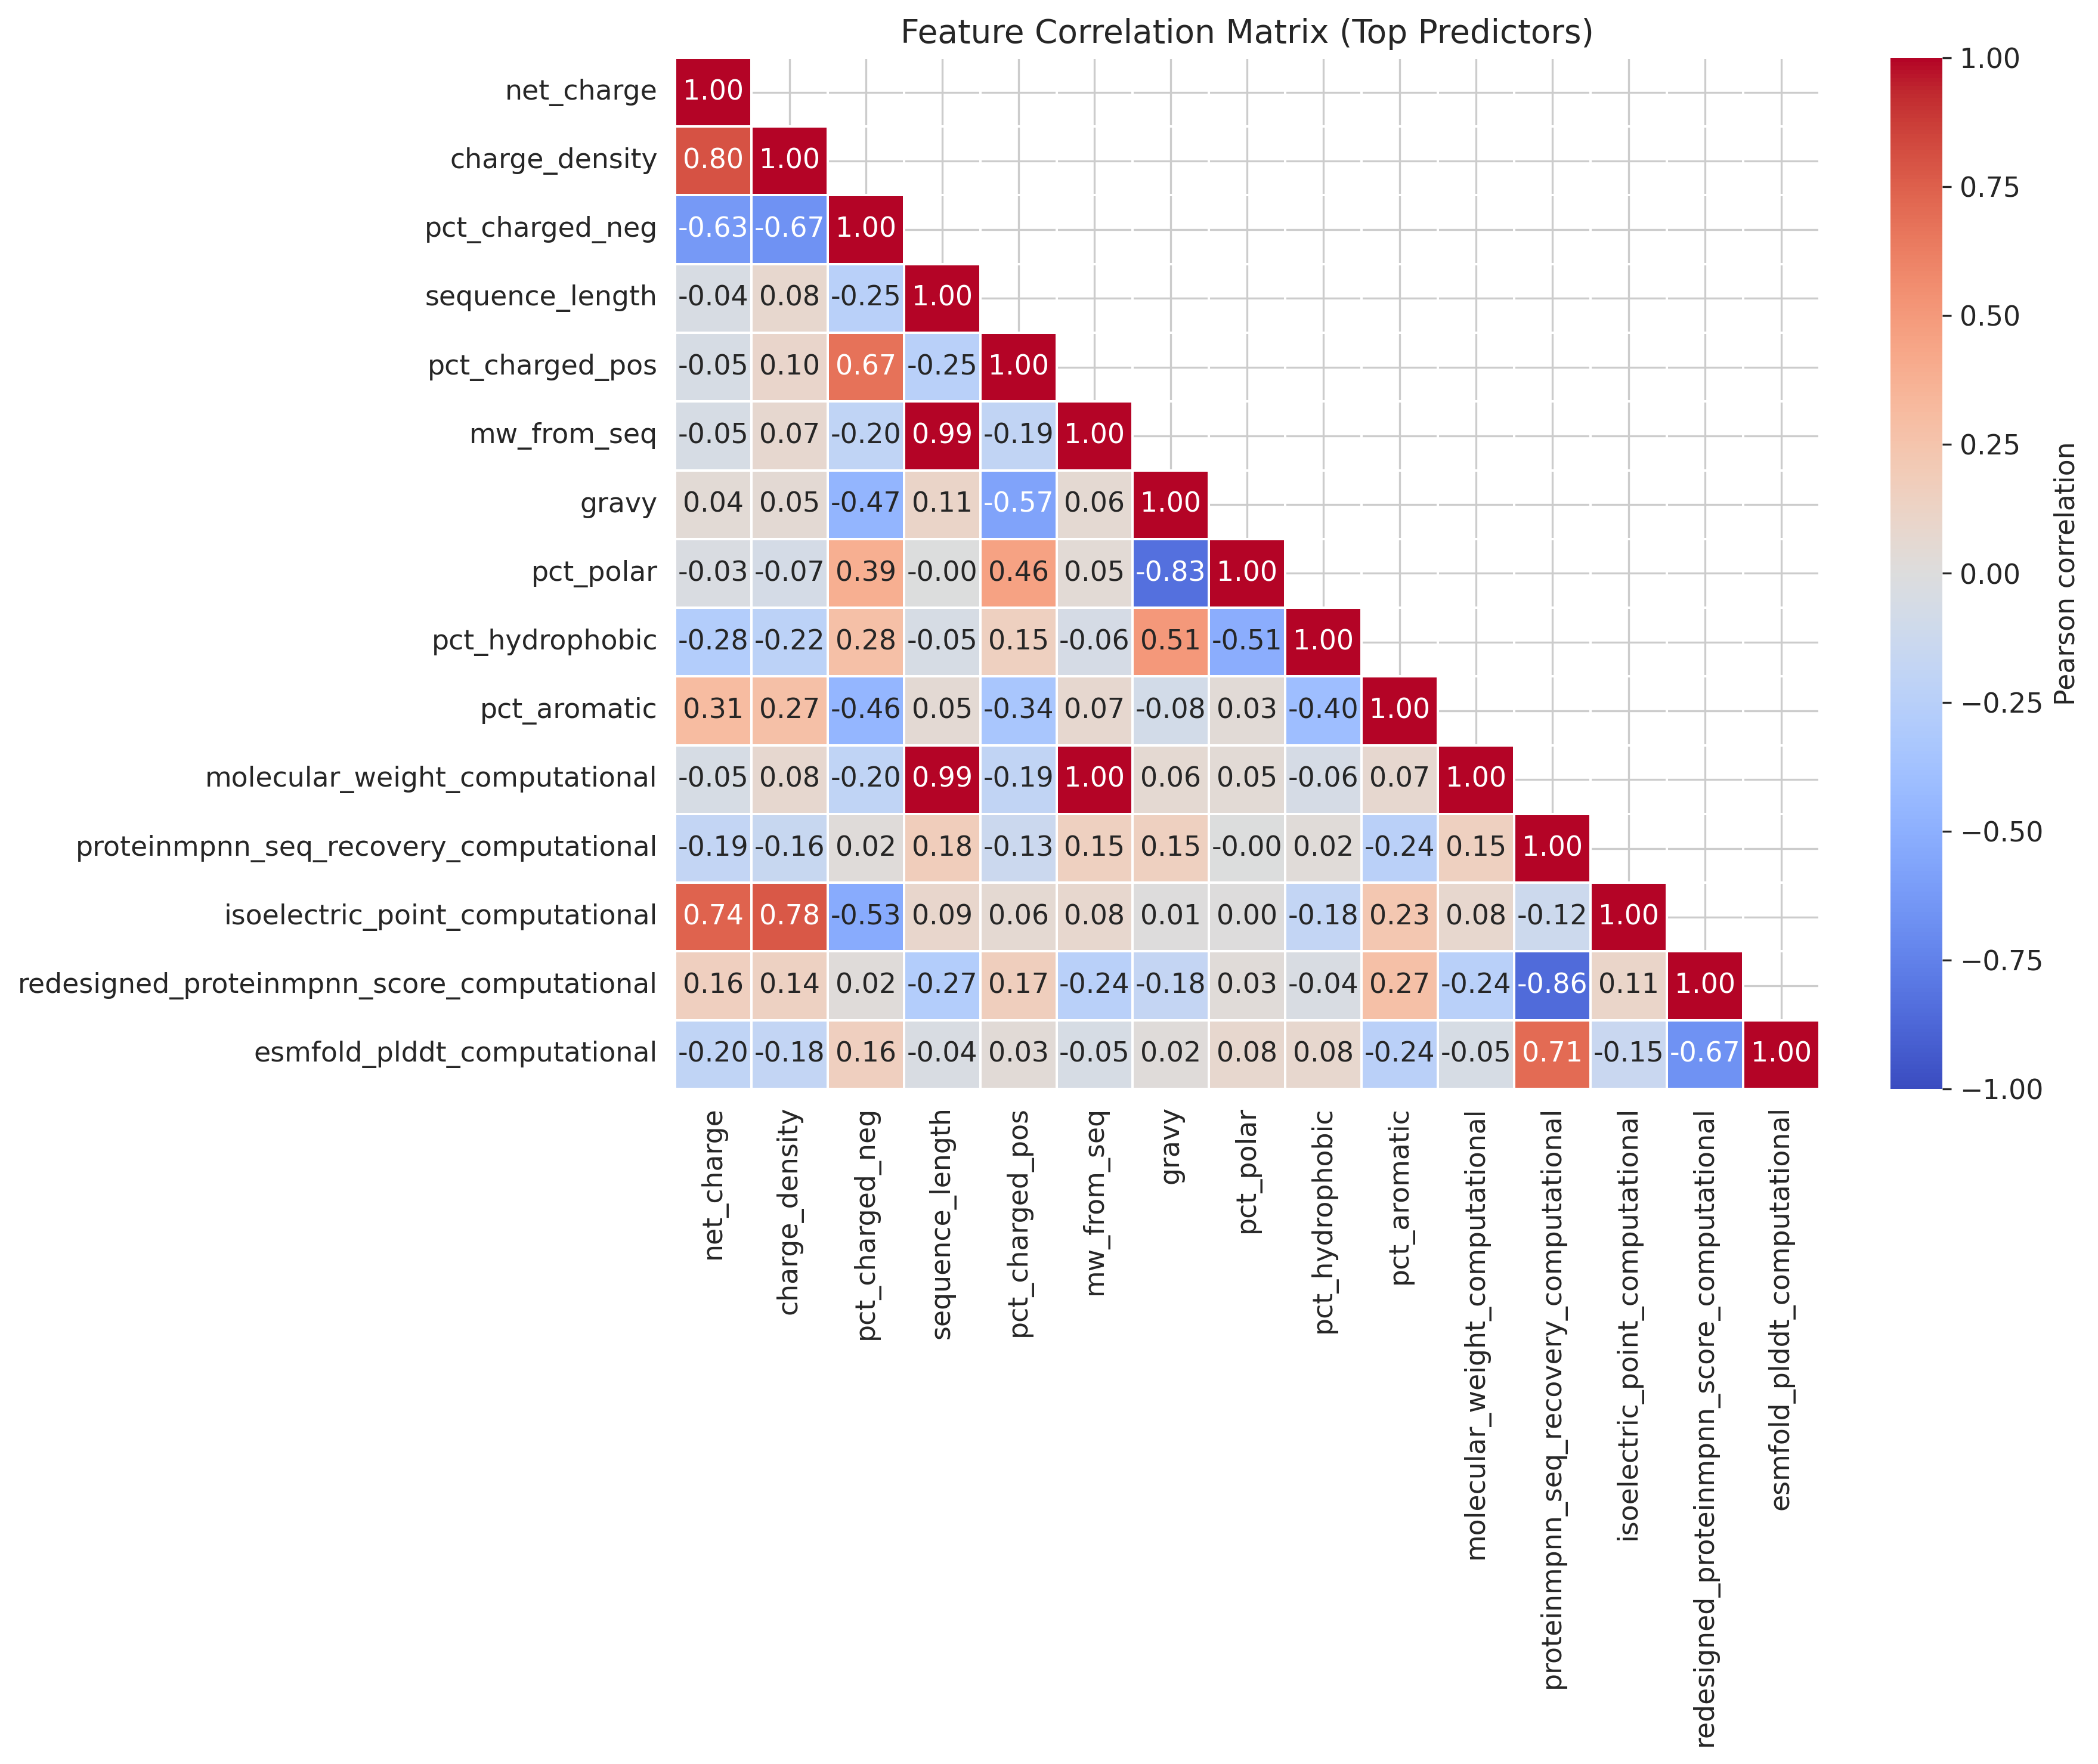
\includegraphics[width=0.85\textwidth]{fig9_correlation_heatmap.png}
\caption{Correlation heatmap for the top 15 features. Strong clusters are visible among structural homology features from different databases.}
\label{fig:heatmap}
\end{figure}

% ======================================================================
\section{Discussion}

\subsection{Comparison with Overath et al.\ (2025)}

Our expanded analysis (5,253 designs, 24 targets) confirms the core conclusions of Overath et al.\ (3,766 binders, 15 targets):

\begin{enumerate}
    \item \textbf{Structure prediction confidence is the most significant universal predictor.} Overath et al.\ reported AF3 ipSAE as the top feature; we find ESMFold pLDDT plays an analogous role on our dataset ($p = 6.9 \times 10^{-11}$), likely because ESMFold predictions were available for more targets.

    \item \textbf{Interaction features outperform individual features.} Our best interaction achieves a 17.3\% AP improvement, comparable to the Overath et al.\ finding that confidence $\times$ physicochemical products are the best predictors.

    \item \textbf{Per-target variability dominates.} AP ranges from 0.10 to 0.95 in our data (0.1 to 1.0 in Overath et al.), confirming that target tractability is the primary source of variation.

    \item \textbf{Greedy selection converges at 2--5 features.} Our greedy selector converges at 2 features, at the lower end of the Overath et al.\ range, consistent with the high intercorrelation among available features.
\end{enumerate}

\subsection{New insights from the expanded dataset}

Several findings emerge from our larger and more diverse dataset:

\textbf{Physicochemical properties are the most consistent cross-target predictors.}
While structure-based scores achieve the largest effect sizes for specific targets, charge-related features (particularly negative charge fraction) appear in the top 5 for the most targets.
This suggests that basic sequence composition provides a target-agnostic baseline that is difficult to improve upon without target-specific information.

\textbf{Sequence identity to known proteins predicts affinity, not just binding.}
Among confirmed binders, sequence identity is by far the strongest predictor of how tightly the design binds ($r = 0.68$ with \pKD), suggesting that evolutionary optimization of binding interfaces is difficult to fully recapitulate de novo.

\textbf{The cross-target AP is modest (0.211).}
When fitting a single model across all targets, AP is only slightly above the baseline rate of 0.179.
This underscores that a universal binding predictor remains elusive; target-specific models or target-specific features (like Boltz2 complex predictions) are needed for practical utility.

\subsection{Practical recommendations}

Based on our analysis, we recommend a tiered approach to computational filtering:

\begin{itemize}
    \item \textbf{Tier 1 --- Universal pre-filters:} ESMFold pLDDT (remove low-confidence designs) and charged residue fraction (consistent discriminator across 6 targets).

    \item \textbf{Tier 2 --- Target-specific scoring:} When available, Boltz2 complex predictions (iPLDDT, shape complementarity, ipSAE) provide the largest effect sizes. Overath et al.\ recommend AF3 ipSAE\textsubscript{min} $> 0.61$ as a threshold.

    \item \textbf{Tier 3 --- Interaction features for enrichment:} TM-score $\times$ charged residue fraction achieves the highest AP (0.326) and should be used to rank designs for experimental testing.

    \item \textbf{Affinity prediction:} Among designs that pass binding filters, prioritize those with higher sequence identity to known proteins for tighter binding.
\end{itemize}

\subsection{Limitations}

Several limitations apply:

\begin{itemize}
    \item \textbf{Dataset composition:} The dataset is dominated by nipah-glycoprotein-g (1,033 samples, 39\% of data) and egfr (770 samples, 29\%), which may bias population-level statistics.

    \item \textbf{Feature availability:} Not all features are available for all targets. Boltz2 complex predictions are only available for targets with pre-computed complex structures, limiting their use as universal features.

    \item \textbf{Design method heterogeneity:} Different targets were designed using different computational pipelines, confounding the comparison of scoring features across targets.

    \item \textbf{Experimental assay variability:} Binding was measured using different assays (SPR, BLI) with different sensitivity thresholds across studies.
\end{itemize}

% ======================================================================
\section{Conclusion}

This analysis of 5,253 de novo protein designs across 24 targets confirms and extends the findings of Overath et al.\ (2025): computational features do predict experimental binding, but modestly and heterogeneously.
Structure prediction confidence (ESMFold pLDDT) is the most universally significant predictor, interaction features combining structural and physicochemical properties improve prediction by 17\%, and per-target variability remains the dominant challenge.
Greedy selection converges at just 2 features, highlighting the high redundancy among available metrics.
Among confirmed binders, sequence identity to known proteins is the strongest affinity predictor ($r = 0.68$), suggesting that evolutionary information remains difficult to replace.

The practical implication is clear: computational scoring can enrich for binders at 3--5$\times$ the random rate, meaningfully reducing experimental costs, but a universal high-confidence predictor remains out of reach.
Target-specific scoring, when available, substantially outperforms target-agnostic approaches.

Code and results: \url{https://github.com/sermare/willitbind}

% ======================================================================
\section*{Acknowledgments}

This analysis builds on the methodology of Overath et al.\ (2025) and uses computational predictions from ESMFold, Boltz2, ProteinMPNN, and Foldseek.

% ======================================================================
\bibliographystyle{unsrtnat}

\begin{thebibliography}{9}

\bibitem{overath2025}
Overath MD, Rygaard ASH, Jacobsen CP, et al.
\newblock Predicting experimental success in de novo binder design: a meta-analysis of 3,766 experimentally characterised binders.
\newblock \textit{bioRxiv}, 2025.
\newblock doi:10.1101/2025.08.14.670059.

\bibitem{watson2023}
Watson JL, Juergens D, Bennett NR, et al.
\newblock De novo design of protein structure and function with {RFdiffusion}.
\newblock \textit{Nature}, 620:1089--1100, 2023.

\bibitem{dauparas2022}
Dauparas J, Anishchenko I, Bennett N, et al.
\newblock Robust deep learning-based protein sequence design using {ProteinMPNN}.
\newblock \textit{Science}, 378(6615):49--56, 2022.

\bibitem{saito2015}
Saito T, Rehmsmeier M.
\newblock The precision-recall plot is more informative than the {ROC} plot when evaluating binary classifiers on imbalanced datasets.
\newblock \textit{PLoS ONE}, 10(3):e0118432, 2015.

\end{thebibliography}

\end{document}
